\documentclass{article}
% if you need to pass options to natbib, use, e.g.:
     \PassOptionsToPackage{numbers, compress}{natbib}
% before loading neurips_2020

% ready for submission
% \usepackage{neurips_2020}

% to compile a preprint version, e.g., for submission to arXiv, add add the
% [preprint] option:
%     \usepackage[preprint]{neurips_2020}

% to compile a camera-ready version, add the [final] option, e.g.:
%     \usepackage[final]{neurips_2020}

% to avoid loading the natbib package, add option nonatbib:
     \usepackage[nonatbib]{neurips_2020}

\usepackage[utf8]{inputenc} % allow utf-8 input
\usepackage[T1]{fontenc}    % use 8-bit T1 fonts
\usepackage{hyperref}       % hyperlinks
\usepackage{url}            % simple URL typesetting
\usepackage{booktabs}       % professional-quality tables
\usepackage{amsfonts}       % blackboard math symbols
\usepackage{amssymb}
\usepackage{nicefrac}       % compact symbols for 1/2, etc.
\usepackage{microtype}      % microtypography
\usepackage{amsmath}
%Graphs
\usepackage{tikz}
\usepackage{pgfplots}
\usepackage[export]{adjustbox}
\usepackage{xcolor,colortbl}
\usepackage[capposition=top]{floatrow}
\hypersetup{
	colorlinks,
	linkcolor = {red!50!black},
	citecolor = {blue!50!black},
	urlcolor = {blue!80!black}
}

\usepackage{lscape}
\usepackage{longtable}
\usepackage{placeins}
\usepackage{floatrow}

\title{Evaluation of Machine Learning in Empirical Asset Pricing}

% The \author macro works with any number of authors. There are two commands
% used to separate the names and addresses of multiple authors: \And and \AND.
%
% Using \And between authors leaves it to LaTeX to determine where to break the
% lines. Using \AND forces a line break at that point. So, if LaTeX puts 3 of 4
% authors names on the first line, and the last on the second line, try using
% \AND instead of \And before the third author name.

\author{%
  David S.~Hippocampus\thanks{Use footnote for providing further information
    about author (webpage, alternative address)---\emph{not} for acknowledging
    funding agencies.} \\
  Department of Computer Science\\
  Cranberry-Lemon University\\
  Pittsburgh, PA 15213 \\
  \texttt{hippo@cs.cranberry-lemon.edu} \\
  % examples of more authors
  % \And
  % Coauthor \\
  % Affiliation \\
  % Address \\
  % \texttt{email} \\
  % \AND
  % Coauthor \\
  % Affiliation \\
  % Address \\
  % \texttt{email} \\
  % \And
  % Coauthor \\
  % Affiliation \\
  % Address \\
  % \texttt{email} \\
  % \And
  % Coauthor \\
  % Affiliation \\
  % Address \\
  % \texttt{email} \\
}

%Graphs
\usepackage{tikz}
\usepackage[export]{adjustbox}
\usepackage{multirow}
\usepackage{array}
\usepackage{multirow}
\usepackage{wrapfig}
\usepackage{float}
\usepackage{colortbl}
\usepackage{pdflscape}
\usepackage{tabu}
\usepackage{booktabs}
\usepackage{threeparttable}
\usepackage{threeparttablex}
\usepackage[normalem]{ulem}
\usepackage{makecell}
\usepackage{xcolor}

%% Macros
\newcommand{\z}[2]{z_{#1, #2}}
\newcommand{\xbf}{\mathbf{x}}
\newcommand{\zVec}[3]{\mathbf{z}_{#1, #2:#3}}
\newcommand{\xVec}[3]{\mathbf{x}_{#1, #2:#3}}
\newcommand{\hVec}{\mathbf{h}}

\begin{document}

\maketitle

\begin{abstract}
	Several recent studies have claimed that machine learning methods provide superior predictive accuracy of asset returns, relative to simpler modelling approaches, and can correctly identify factors needed to price portfolio risk. Herein, we demonstrate that this performance is critically dependent on several features of the data being analysed; including, the training/test sample split, the frequency at which the data is observed, and the chosen loss-function. In contrast to existing studies, which claim that neural nets provide superior predictive accuracy, through a series of realistic examples that mimics the stylized facts of asset returns, we demonstrate that neural methods are easily outperformed by simpler methods, such as random forests and elastic nets.
\end{abstract}

\section{Introduction}
The dominance of machine learning methods in terms of predictive accuracy has now begun to filter into the application and assessment of asset pricing. The most common application of machine learning methods within finance are for portfolio construction, asset price prediction, and factor selection. 

Several studies have now used machine learning techniques to analyze the cross-section of asset returns and produce portfolios that can capture nonlinear information in the cross-section of asset returns. Mortiz and Zimmermann (2016) use tree-based methods in an attempt to understand which firm-level characteristics best predict the cross-section of stock returns, where this information can then be used within portfolio sorting to help mitigate risk. Similarly, Messemer (2017) uses deep feedforward neural nets (DFNs) to construct portfolios and predict the returns across a cross-sections of US asset returns. While Messemer (2017) demonstrates that such DFNs can better capture nonlinear information, and outperform portfolios generated from linear benchmarks, the author does not claim that deep learning methods are the best methods to exploit these nonlinear interactions. 

In addition, several studies have now suggested that machine learning methods can produce better predictions of asset returns (\cite{gu_empirical_2018}, \cite{hsu_finding_2014} and \cite{feng_deep_2018}). In particular, the results of Gu et al. (2019) suggest that, in terms of predictive performance, as measured by an out-of-sample $R^2$,  tree-based methods and shallow neural nets can provide superior predictive accuracy over other machine learning methods and simpler model-based approaches. This finding is born out both in terms of simulated data, and an empirical example with monthly returns data from 1957 to 2016. \cite{gu_empirical_2018} attribute this to machine learning's ability to evaluate and consider non-linear complexities among factors that cannot be feasibly achieved using traditional techniques. 

Similarly, work by Kozak et al, (2018), Freyberger et al. (2018), Feng et al., (2019) and Rapach and Zhou (2013), demonstrate that machine learning methods can ``systematically evaluate the contribution to asset pricing of any new factor'' used within an existing linear asset pricing structure. In addition, Gu et al. (2019) use variable importance metrics to quantify the differential impact of factors across a large set of possible factors available for asset pricing. As such, machine learning methods can be used, \textit{en masse}, to consistently evaluate the ability of various factors to help price portfolio risk. Such work is particularly useful given the literature's seeming obsession with the XXX and constructing such factors: as of 2014, quantitative trading firms were using 81 factor models (Hsu and Kalesnik, 2014), while Harvey and Liu (2019) currently document that well over 600 different factors have been suggested in the literature. 

While the above studies all demonstrate the potential benefits of machine learning methods within empirical finance, it is unclear whether the findings in these papers are easily generalizable to: one, different training and validation periods; two, different sampling frequencies, which result in stock returns with significant different characteristics (e.g., daily volatility is significantly higher than monthly volatility); and three, different loss-measures of predictive accuracy. The answer to such questions are particularly pertinent given that the machine learning literature has already documented the difficulties of certain methods, including those references above, in dealing with data that displays the stylized facts of asset returns. For instance, methods such as penalized regression and tree-based models assume a form of conditional independence between observations, which is violated by the state dependence that exists within, and across, asset returns. In addition, it has already been noted that training more standard types of neural networks, such as the feed forward kind considered in Gu et al, becomes particularly difficult when data displays strong dependence, (\cite{bengio_learning_1994}). In addition, more complex machine learning approaches require extremely large amounts of data, as well as specialized sample splitting and cross-validation schemes, to deal with possible model over-fitting. 

In some ways, existing applications of machine learning to empirical asset pricing have either over-looked, downplayed, or simply ignored the importance of the above issues. For example, Messemer (2017) and \cite{feng_deep_2018} use cross validation as part of their model building procedures, thereby destroying the temporal ordering of data. In addition, \cite{gu_empirical_2018} and Messemer (2017) produce models using training samples that end much earlier than the data sets which they ultimately produce forecasts for: in the case of Messemer (1970), the training period ends in 1981, while the  which ends in the 1970s to ultimately produce forecasts for the most recent 30 years; in the case of \cite{gu_empirical_2018}, the training ends in the 1970s, with predictions ultimately produced only for the period of returns from 1987-2016.  This is particularly worrying as the factors driving daily or monthly returns in the 1980s, are starkly different than those driving returns in, say, 2001 onwards. However, both of these papers suggest that the training and validation sets used for the various methods does not impact the test set results. 

While some combination of machine learning methods can undoubtedly lead to better performance than simpler model-based solutions, a more systematic treatment on the ability of these methods to 1) accurately detect significant factors; and 2) accurately predict returns according to a range of loss measures, must be formulated before researchers can rely on such methods in practice. The goal of this paper is to bridge this gap and thereby provide a systematic, rigorous, realistic, and reproducible study on the performance of several machine learning methods that have been used in empirical asset pricing. 

First, through a rigorous simulation study, which captures the stylized facts of asset returns, we give an in-depth comparison of several machine learning methods used in the literature. The simulation study explicitly explores how different aspects of financial data such as persistence in regressors, cross sectional correlation and different complexities of data generating process can affect a method's ability to: 1) accurately predict future returns across a range of loss measures; and 2) correctly identify the significant factors driving returns. In contrast to existing findings, in this realistic simulation design, we find that neural network procedures, such as feedforward nets, LSTM (CITE), and DeepAR models (CITE), are among the worst performing methods, while tree-based methods and elastic net are among the best performing methods. We also demonstrate that this result is consistent across various levels of volatility, cross-sectional correlation, return signal, and different loss functions. In addition, we demonstrate that elastic net and tree-based methods also outperform neural net based approach in terms of correctly identifying significant factors.     

Next, we validate these findings using a empirical data set of asset returns that considers quarterly individual price data from CRSP for all firms listed in the NYSE, AMEX and NASDAQ. The starting period of the data is January first 1957 (starting date of the S\&P 500) and the ending date is December 2016, totalling 60 years. A set of 549 possible factors are used to explain the cross-section of returns. We pay careful attention to the training and test split, and only use the last fourteen years of quarterly returns to evaluate the different machine learning methods. The results found in the empirical study agree completely with those in the aforementioned simulation study: across all machine learning methods, neural net based procedure perform the worst across various loss functions, while tree-based methods and elastic net perform the best. 

The results of this study suggest that great care and diligence is required if one wishes to implement machine learning methods within empirical finance. Indeed, our results suggest that the efficacy of machine learning methods within empirical finance depends are highly-dependent on the samples used for training and testing, the loss functions used for evaluation, and the specific nature of the data series one wishes to predict. As such, while potentially quite useful in empirical finance, machine leaning methods are not necessarily a panacea to correctly predict future asset prices or to correctly disentangle which factors are relevant. 

The remainder of the paper is organized as follows.... 

\section{Model and Methods}
\subsection{Statistical Model}
In this section we briefly discuss the statistical model considered for asset returns. Excess monthly returns on asset $i$, $i=1,\dots,n$, at time $t$, $t=1,\dots,T$, are assumed to evolve in an additive fashion:
%% In the case of LSTM and DeepAR, the expectation is conditional on z_t, not z_it (ie they try to leverage information from across the entire cross section to produce predictions)
\begin{equation}\label{eq:model}
r_{i, t+1} = E(r_{i, t+1} | \mathcal{F}_t) + \epsilon_{i, t+1},\;\;E(\epsilon_{i, t+1}|\mathcal{F}_{t})=0
\end{equation} where $\mathcal{F}_t$ denotes the observable information at time $t$, and $\epsilon_{i,t+1}$ is a martingale difference sequence (hereafter, mds). We further consider that the conditional mean of returns is an unknown function of a $P$-dimensional vector of features, assumed measurable at time $t$, such that 
\begin{equation}
E(r_{i, t+1} | \mathcal{F}_t) = g(z_{i,t})
\end{equation} 

The features, or predictors, $z_{i,t}$ are assumed to be composed of time-$t$ information, and depends only the characteristics of stock $i$. It is not assumed that all $z_{i,t}$ are present within the function $g(\cdot)$ across all $i$ units. That is, the function $g(\cdot)$ need not depend on the same $z_{i,t}$ as $i$ varies. The assumption that the information set can be characterized by the variables $z_{i,t}$ without dependence on the $j\neq i$ return units, is reasonable given that the collection of $z_{i,t}$ is rich enough. 

In what follows, we represent  the space of possible features as the Kronecker product of two pieces
\begin{equation}
\label{kronecker_equation}
z_{i,t} = x_t \otimes c_{i,t}
\end{equation}where the variables \( c_{i,t} \) represent a \( P_c \times 1 \) vector of individual-level characteristics for return \(i\), and \(x_t\) represents a $P_x \times 1$ vector of macroeconomic predictors, and $\otimes$ represents the Kronecker product. Thus, for $P = P_c\cdot P_x$, $z_{i,t}$ represents a $P \times 1$ feature space that can be used to approximate the unknown function $g(\cdot)$.

\subsection{Methods}Given features $z_{i,t}$, the goal of any machine learning method is to approximate the unknown function $g(\cdot)$ in \ref{eq:model}.  Broadly speaking, how different ML methods choose to approximate this function depends on three components:
\begin{enumerate}
	\item the model used to make predictions,\footnote{The model used by the ML method need not correspond to the statical models assumed to describe the data. Herein, our goal will not be to asses the ``accuracy'' of the statistical model, but to determine how different ML methods accurately determine the salient features of this model. }
	\item the regularization mechanism employed to mitigate over-fitting; 
	\item a loss function that penalized poor predictions. 
\end{enumerate}

%It is important to note that the model used by the ML method need not correspond to the statical models assumed to describe the data. In general, the specification of the statistical model entails uncertainty, however, the model a given ML method uses to generate prediction is known, possibly up to unknown functions. In what follows, our goal will not be to asses the ``accuracy'' of the statistical model, but to determine how different ML methods accurately determine the salient features of this model.   

To ensure the results of ML different methods will be comparable, we fix both the regularization mechanisms and loss functions used within each method, and allow only the models used for prediction to vary. This approach seeks to ensure that performances in one method, relative to another, are based on the model structure and not to some feature of how the models were fit. To this end, we first discuss points 2. and 3. above, and then briefly present the models used for our comparison. 
\paragraph{Loss functions:}The choice of loss function used to fit the ML methods is instrumental in the methods' ultimate performance. Herein, we consider two separate loss functions: Mean Absolute Error (MAE) and Mean Squared Error (MSE):
\begin{equation*}
\text{MAE} = \frac{1}{n} \sum_{j = i}^{n} |y_j - \hat{y_j}|\text{ and }
\text{MSE} = \frac{1}{n} \sum_{j = i}^{n} \left( y_j - \hat{y_j}\right) ^2,
\end{equation*}We consider both loss functions since MAE is less sensitive to outliers in the data which financial returns are known to exhibit, and which are caused by extreme market movements. Given this, we expect MAE to  produce predictive results that are more robust to such outlier events. 

\paragraph{Mitigating over-fitting:}ML methods guard against over-fitting by emphasizing out-of-sample performance. To this end, observed data is split into ``training”, ``validation'' and ``test'' sets. Since returns data is intrinsically dependent, when constructing such a split we must consider a schema that respects this dependence structure. 

Throughout our experiments/applications, to balance computation and accuracy, we use a  hybrid ``rolling window"  and ``recursive'' approach to training/validation/test splits: for each model refit, the training set is increased by one year observations, i.e., $12$ monthly observations; the validation set is fixed at one year and moves forward (by one year) with each model refit; predictions are generated using that model for the subsequent year.

%This schema is chosen as it strikes a reasonable balance between computational complexity, and predictive accuracy, while allowing newer information to enter into, and have reasonable weight within, the subsequent predictions.  

\paragraph{Models} The remaining specification for the ML methods is the chosen model used to generate predictions. Herein, we consider a host of different models: including elastic net (Hastie et al., XXX), Random forest (XXX), feed-forward neural nets (XXX), LSTM (XXX), FFORMA (XXX) and DeepAR models (XXX). To keep the details as brief as possible, we give full details on each model and certain features of its implementation used in this work in the appendix. For each of the different methods, we consider two variants, one based on the MAE loss and one based on the MSE loss. 

\subsection{Model evaluation measures}
\paragraph{Predictive accuracy}

Predictive performance for individual excess returns are assessed using Mean Absolute Error (MAE), Mean Squared Error (MSE) (evaluated over the test set) and an out-of-sample $R^2$ measure. While  out-of-sample $R^2$ is a common measure, there is no universally agreed-upon definition. As such, we explicitly state the version employed herein as
\begin{align}
R^2_{OOS} &= 1 - \frac{\sum_{(i, t)\in\mathcal{T}_3}(r_{i, t+1} - \widehat{r}_{i, t+1})^2}
{\sum_{(i, t)\in\mathcal{T}_3} \left( r_{i, t+1} - \bar{r}_{i, t+1} \right) ^2}
\end{align}
where $\mathcal{T}_3$ indicates that the fits are only assessed on the test sub-sample, which is never used for training or tuning.

Since $R^2$ is based on in-sample-fit of a linear model, this measure is less meaningful for most of the ML methods considered in in this paper. However, we report this measure since this measure has also been considered in other applications of ML to empirical finance (see, e.g., Gu et al., 2019). 
\paragraph{Factor Selection}
An important aspect of empirical finance is the understanding of which features drive risk. That is, which features are explicitly represented within $z_{i,t}$ and can thus be used to help price risk using equation \ref{eq:model}. To this end, we define a simple variable importance (VI) measure to be applied across all ML methods in this research. To this end, we mirror the measure produced in \cite{gu_empirical_2018} and define $VI_j$ as the reduction in predictive $R^2$ from setting all values of predictor $j$ to 0, while holding the remaining model estimates fixed. Each $VI_j$ is then normalized to sum to 1. 

However, as $VI_j$ can sometimes be negative, we shift $VI_j$ by the smallest $VI_j$ plus a small constant, then dividing by this sum to alleviate numerical issues\footnote{This mechanism was chosen because the other popular normalization mechanism ``softmax" was observed to be unable to preserve the distances between each original $VI_j$, making discernment between each $VI_j$ difficult.}. The resulting VI measure is then. 
\begin{equation}
VI_{j, norm} = \frac{VI_j + \operatorname{min}(VI_j) + o}
{\Sigma VI_j + \operatorname{min}(VI_j) + o} \quad ; \quad o = 10^{-100}
\end{equation}

%%%%%%%%%%%%%%%%%%%%%%%%%%%%%%%%%%%%%%%%%
\section{Simulation study}
We begin with the simulation study as a way to explore how machine learning performs with regards to the stylized facts of empirical returns in a controlled environment. We simulate according to a design which incorporates low signal to noise ratio, stochastic volatility in errors, persistence and cross sectional correlation in regressors. Our specification is a latent factor model for excess returns $r_{t+1}$, for $t=1, \dots, T$:
\begin{align}
r_{i, t+1} &= 
g\left(z_{i, t}\right) + \beta_{i,t+1}v_{t+1} + e_{i, t+1}; 
\enspace z_{i, t} = \left(1, x_{t}\right)^{\prime} \otimes c_{i, t}, 
\enspace \beta_{i, t} = \left(c_{i 1, t}, c_{i 2, t}, c_{i 3, t}\right) \\ 
e_{i, t+1} &= 
\sigma_{i, t+1} \varepsilon_{i, t+1}; \\
\operatorname{log} (\sigma^2_{i,t+1}) &= 
\omega + \gamma \operatorname{log} (\sigma^2_{t}) + \sigma_{u}u;
\quad u \sim N(0, 1)
\end{align}
where $v_{t+1}$ is a $3\times 1$ vector of errors, $w_{t+1} \sim N(0, 1)$,  $\varepsilon_{i,t+1} \sim N(0, 1)$ scalar error terms, matrix $C_t$ is an $N\times P_c$ matrix of latent factors, where the first three columns correspond to $\beta_{i,t}$, across the $1\leq i\leq N$ dimensions, while the remaining $P_c-3$ factors do not enter the return equation. The $P_x\times1$ vector $x_t$ is a $3 \times 1$ multivariate time series, and $\varepsilon_{t+1}$ is a $N\times 1$ vector of idiosyncratic errors. The parameters of these were tuned such that the annualized volatility of each return series was approximately 22\%, as is often observed empirically.
%%%%%%%%%%%%%%%%%%%%%
\paragraph{Simulating characteristics}
We build in correlation across time among factors by drawing normal random numbers for each $1\leq i\leq N$ and $1\leq j\leq P_{c}$, according to :
\begin{equation}
\overline{c}_{i j, t} = \rho_{j} \overline{c}_{i j, t-1}+\epsilon_{i j, t} ;
\quad \rho_{j} \sim \mathcal{U} \left( 0.5, 1 \right) 
\end{equation}
We then build in cross sectional correlation:
\begin{align}
\widehat{C}_{t}&=L\overline{C}_{t} ; \quad B = LL' \\
B:&=\Lambda\Lambda' + 0.1\mathbb{I}_{n}, \quad
\Lambda_i = (\lambda_{i1}, \dots, \lambda_{i4}), \quad
\lambda_{ik}\sim N(0, \lambda_{sd}), \; k=1, \dots, 4
\end{align}
where $B$ serves as a variance covariance matrix with $\lambda_{sd}$ its density, and $L$ represents the lower triangle matrix of $B$ via the Cholesky decomposition. $\lambda_{sd}$ values of 0.01, 0.1 and 1 were used to explore increasing degrees of cross sectional correlation.
Characteristics are then normalized to be within $[-1, 1]$ for each $1\leq i\leq N$ and for $j=1, \dots, P_{c}$ via:
\begin{equation}
c_{i j, t} = \frac{2}{n+1} \operatorname{rank}\left(\hat{c}_{i j, t}\right) - 1.
\end{equation}
%%%%%%%%%%%%%%%%%%%%%%
\paragraph{Simulating macroeconomic series}
We consider a Vector Autoregression (VAR) model for $x_{t}$, a $3 \times 1$ multivariate time series \footnote{More complex specifications for $A$ were briefly explored, but these did not have a significant impact on results.}:
\begin{flalign*}
x_{t} = Ax_{t-1}+u_t; 
\quad A = 0.95 I_3;
\quad u_t \sim N\left( \mu = (0, 0, 0)' , \Sigma = I_3
\right) 
\end{flalign*}
\paragraph{Simulating return series}
We consider three different functions for $g(z_{i, t})$:
\begin{align}
(1)\; & g_1 \left(z_{i, t}\right)=\left(c_{i 1, t}, c_{i 2, t}, c_{i 3, t} \times x_{t}'[3,]\right) \theta_{0} \\
(2)\; & g_2 \left(z_{i, t}\right)=\left(c_{i 1, t}^{2}, c_{i 1, t} \times c_{i 2, t}, \operatorname{sgn}\left(c_{i 3, t} \times  x_{t}'[3,]\right)\right) \theta_{0} \\
(3)\; & g_3 \left(z_{i, t}\right) = \left(1[c_{i3,t}>0],c_{i 2, t}^{3}, c_{i 1, t} \times c_{i 2, t}\times 1[c_{i3,t}>0], \text{logit}\left({c}_{i3, t} \right)\right) \theta_{0}
\end{align}
where $x_{t}'[3,]$ denotes the third element of the $x_{t}'$ vector.
%%%%%%%%%%%%%%%%%%%%%%%%%
$g_1 \left(z_{i, t}\right)$ allows the characteristics to enter the return equation linearly, and $g_2 \left(z_{i, t}\right)$ and $g_3 \left(z_{i, t}\right)$ allow the characteristics to enter the return equation interactively and non-linearly. \footnote{($g_1, g_2$ correspond to the simulation design used by \cite{gu_empirical_2018}.)} $\theta^0$ was tuned such that the predictive $R^2$ was approximately 5\%.

The simulation design results in $3 \times 3 = 9$ different simulated datasets, each with $N = 200$ stocks, $T = 180$ periods and $P_c = 100$ characteristics. Each design was simulated 10 times to assess the robustness of machine learning algorithms, with the number of simulations kept low for computational feasibility. We employ the hybrid data splitting approach with a training:validation length ratio of approximately 1.5 and a test set that is 1 year in length. 

%% Other schemes in the forecasting literature such as using an ``inner" rolling window validation loop to find the best hyperparameters on average, finally aggregating them in an ``outer" loop for a more robust error were considered but not implemented for a variety of reasons. Firstly, many of the models were computationally too intensive for this to be feasible. More importantly, during the model fitting process it was observed that the optimal hyperparameters for the different rolling windows were highly unstable (see Appendix). Thus, this would have made the selection of the best hyperparameters on average across all windows significantly less meaningful.

%%%%%%%%%%%%%%%%%%%%%%%%%%%%%%%%%%%%%%%%%%%%%%%%%%%%%%%%%%%%%%%%%%%%%%%%%%%%%%%%%%%%%%%%%%%%%%%%%%%%%%%%%%%%%%%%%%
\subsection{Simulation Study Results}

\paragraph{Prediction Performance}
In general, elastic nets are the best performing model, followed closely by random forests, then neural networks. All machine learning models were unaffected by cross sectional correlation in terms of prediction performance, and typically had better performance when fitted with respect to quantile loss. Random forests only outperformed the elastic nets on highly non-linear specifications. The neural network models were not observed to outperform any of the machine learning models. 

This is in stark contrast to the linear models, which are severely affected by both increasing non-linearities cross sectional correlation. This result is consistent across all loss metrics.

Machine learning models fitted with respect to minimizing MAE (quantile loss) generally perform better, even when evaluated against MSE loss metrics. This is not a surprising result, especially considering the stochastic error design which introduces significant shocks to the returns process. Though the actual difference between the loss metrics between the penalized linear models, random forests and neural networks are very small, when considering the consistency of the results across numerous Monte Carlo simulations, the differences in prediction performance, though small, is robust and significant.

\begingroup\fontsize{6}{8}\selectfont

\begin{longtable}[t]{cccccccc}
\caption{\label{tab:}Top Models in Simulation Study}\\
\toprule
\multicolumn{1}{c}{ } & \multicolumn{1}{c}{ } & \multicolumn{3}{c}{Test MAE} & \multicolumn{3}{c}{Test MSE} \\
\cmidrule(l{3pt}r{3pt}){3-5} \cmidrule(l{3pt}r{3pt}){6-8}
Corr & model & g1 & g2 & g3 & g1 & g2 & g3\\
\midrule
\endfirsthead
\caption[]{Top Models in Simulation Study }\\
\toprule
\multicolumn{1}{c}{ } & \multicolumn{1}{c}{ } & \multicolumn{3}{c}{Test MAE} & \multicolumn{3}{c}{Test MSE} \\
\cmidrule(l{3pt}r{3pt}){3-5} \cmidrule(l{3pt}r{3pt}){6-8}
Corr & model & g1 & g2 & g3 & g1 & g2 & g3\\
\midrule
\endhead
\
\endfoot
\bottomrule
\endlastfoot
 & ELN.MAE & 0.0345786 & 0.0361950 & 0.0353345 & 0.0025652 & 0.0026882 & 0.0026210\\

 & RF.MAE & 0.0354594 & 0.0354204 & 0.0355399 & 0.0026434 & 0.0026305 & 0.0026446\\

 & NN2.MAE & 0.0359604 & 0.0369206 & 0.0363047 & 0.0026786 & 0.0027474 & 0.0026996\\

 & NN1.MAE & 0.0358939 & 0.0368335 & 0.0363352 & 0.0026718 & 0.0027396 & 0.0027028\\

\multirow{-5}{*}{\centering\arraybackslash \rotatebox{90}{0.01}} & NN3.MAE & 0.0358164 & 0.0369345 & 0.0364712 & 0.0026697 & 0.0027491 & 0.0027181\\
\cmidrule{1-8}
 & ELN.MSE & 0.0346142 & 0.0362761 & 0.0354437 & 0.0025676 & 0.0026980 & 0.0026300\\

 & RF.MAE & 0.0359158 & 0.0356434 & 0.0360529 & 0.0026747 & 0.0026445 & 0.0026786\\

 & NN5.MAE & 0.0370087 & 0.0372705 & 0.0374132 & 0.0027744 & 0.0027832 & 0.0027916\\

 & NN4.MSE & 0.0373820 & 0.0368966 & 0.0373542 & 0.0028051 & 0.0027505 & 0.0027970\\

\multirow{-5}{*}{\centering\arraybackslash \rotatebox{90}{1}} & NN3.MAE & 0.0372849 & 0.0370382 & 0.0371925 & 0.0027940 & 0.0027652 & 0.0027753\\*
\end{longtable}
\endgroup{}
% Across all specifications with a stochastic volatility component, we observe a decrease in prediction performance as the sample size increased according to the expanding window approach implemented. This is likely due a larger sample having a higher chance to experiences external shocks due to the stochastic volatility process, and thus a higher chance to experience large outliers in the training sample, leading to worse prediction performance. This indicates that machine learning performs poorly when the training data supplied contains more large outliers, and is still sensitive to such outliers even with the use of regularization and robust loss functions.

% Focusing on the neural networks, we clearly see that they do not outperform any of the other machine learning models, even when the underlying data generating process is non-linear. This directly contradicts the result which \cite{gu_empirical_2018} find, even when considering the design with no cross sectional correlation and stochastic volatility (top row in graphs), which corresponds to their exact specification but with a multivariate macroeconomic series. We also find consistent evidence that deeper architectures provide better prediction performance, another result which contradicts \cite{gu_empirical_2018}'s conclusions that shallow learning may be better.

\paragraph{Factor Importance}
We observe that the elastic net outperforms all other models consistently in terms of assigning the correct relative importance to the true underlying regressors, \footnote{($c_1.\text{constant}$, $c_2.\text{constant}$ and $c_3.x_3$ for $g1$ and $g_2$ specifications, and $c_1.\text{constant}$, $c_2.\text{constant}$ and $c_3.\text{constant}$ for $g_3$)} even in settings with high cross sectional correlation. 

Elastic net models perform the best at identifying the true data generating regressors, and  this appears to be mostly robust regardless of cross sectional correlation, though their performance worsens as the data generating process becomes more non-linear. On more difficult specifications, the elastic net models are conservative and typically identify a single regressor as importance - most apparent on the $g_2$ specification. Occasionally, the elastic nets identified the incorrect covariates, assigned them low relative importance.

The random forests and to a lesser extent the neural networks also correctly identified the correct underlying regressors, but struggled with adequately discerning relative importance among correlated regressors. This was became more apparent as the degree of cross sectional correlation increased (see decreasing relative importance of true underlying regressors in Figures \ref{fig:rf_sim_vi} and \ref{fig:nn_sim_vi} in Appendix). 

%% Intuitive explanation of why random forests struggle with relative discernment - not sure if necessary
%In the case of the random forests, this is to be expected, likely due to how the random forest algorithms work. The random forest algorithm is an ensemble of tree models, with each tree model only having access to a subset of all available predictors. If this subset does not include the true data generating predictor, then that particular tree will likely select the predictors which have the highest correlation with the true data generating predictor instead. Thus, the resulting ensemble model is likely to believe that cross sectionally correlated predictors are important, relative to the true underlying regressor. Due to the complexity of the neural networks, there does not exist a similar intuitive explanation for their factor selection ability.

%% Need to make these plots even smaller somehow, or omit one or two of them
%% Ended up faceting and mushing these graphs all together
\begin{figure}
	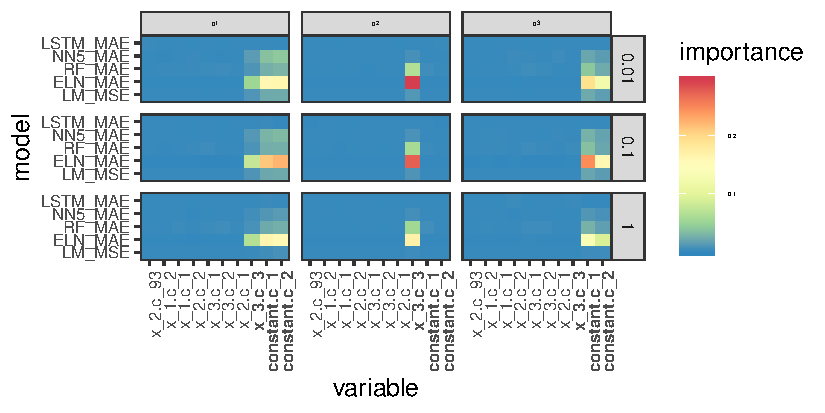
\includegraphics[max size = {\textwidth}{0.4\textheight}]{../../Results/simulation/graphics/simulation_all_g_vi.pdf}
	\caption{Simulation variable importance, faceted by simulation specification}
\end{figure}

The linear models unsurprisingly struggled with factor significance analysis with respect to both increasing cross sectional correlation non-linearities. This highlights the non-robustness and ineffectiveness of using traditional linear regression as documented by the literature; linear models were consistently observed to identify irrelevant regressors as important, especially as the degree of cross sectional correlation increased. Considering that the graphs represent the averaged variable importance metrics over different simulation realisations, this means that on a single simulation realization, the performance of linear models is significantly worse.

%% Brief other notes that are not too important

% The overall high performance of the elastic net models may be somewhat surprising given its relative simplicity compared to other machine learning models. However, when recalling that elastic net models are the only machine learning models which are specifically noted to perform well on datasets with high degrees of multicollinearity, the result is perhaps less surprising. Indeed, random forest and neural network models are only noted to be better at capturing non-linear relationships in independent and identically distributed data, a property which we observe on the non-linear specification, and only for the random forests.

% Of particular note are the instability of the machine learning models' hyperparameters across different training samples. For the elastic nets, the optimal value for $\alpha$ is generally 1 (corresponding to LASSO and thus a sparse representation), but it was not uncommon to observe $\alpha$ values swinging between values close to 0 (corresponding to ridge regression, and thus a dense representation) to 1 as the training sample moved forwards in time. As the penalized linear models consistently performed the best and still remained able to correctly identify the true covariates this is not a large issue, but it should be noted that this can lead to interpretation issues. For the random forests, it was similarly observed that the optimal value for $mtry$ (the number of variables subsetted) and $nodesize$ was highly non-robust. Again, given that the final prediction performance was consistent this is not a large issue, but can lead to some interpretation issues.

\section{Empirical analysis}
We conduct an empirical study as a final way to corroborate the findings of the properties of machine learning models which we observed in the simulation study. Though our simulation study was aimed at capturing the main features of observed data, the underlying data generating process for empirical returns is unknown. This study thus acts as a robustness check as to how machine learning performs on real world data, which can be significantly more complex and noisy than simulated contexts. 

Importantly, we find that our findings from the simulation study are largely corroborated for empirical returns data.

\subsection{Data}
We begin by obtaining monthly individual price data from CRSP for all firms listed in the NYSE, AMEX and NASDAQ, starting from 1957 (starting date of the S\&P 500) and ending in December 2016, totalling 60 years. To build individual factors, we construct a factor set based on the cross section of returns literature. This is the same data used in \cite{gu_empirical_2018}. We restrict our dataset to begin from 1993 Q3 and end on 2016 Q4 to alleviate data quality issues. Our individual factor set contains 94 characteristics: 61 updated annually, 13 updated quarterly and 20 updated monthly \footnote{The dataset also included 74 Standard Industrial Classification (SIC) codes, but these were omitted due to their inconsistency, and inadequateness at classifying companies, as noted by WRDS}.

% Begin Cleaning

% the dataset was filtered such that only stocks traded primarily on NASDAQ were included (using the PRIMEXCH variable from WRDS). Then, penny stocks (also referred to as microcaps in the literature) with a stock price of less than \$5 were filtered out, as is commonly done in the literature to reduce variability. Stocks without a share code of 10 or 11 (referring to equities) were filtered out, so that securities that are not equities were not included (such as REITs and trust funds). The dataset is provided in a monthly format, which means that many of the factors which are updated only quarterly or annually have very low levels of variability, which can lead to misleading results in the model fitting process. 

We detail our cleaning procedure of this dataset. To reduce the size of the dataset and increase feasibility, we only consider non-penny equities traded primarily on the NASDAQ. To achieve a balance between having a dataset with enough data points and variability among factors, the dataset was converted to a quarterly format. Quarterly returns were then constructed using the PRC variable according to:
\begin{equation}
RET_t = (PRC_t - PRC_{t-1})/PRC_{t-1}
\end{equation}
We allow all stocks which have a quarterly return to enter the dataset, even if they disappear from the dataset for certain periods. This was primarily done to reduce survivorship bias in the dataset, and also allows for stocks which were unlisted and relisted again to feature in the dataset. \footnote{To deal with missing data, any characteristics that had over 20\% of their data missing were omitted. Remaining missing data were then imputed using their cross sectional medians for each year. See Appendix for more details.}

%% Gu et al has the missing data part as a footnote - trying that approach here

% This has the obvious drawback of introducing some bias in the dataset, as attrition in the dataset is likely to be non-random and correlated with the stocks' returns. 

% The sic2 variable, corresponding to the stocks' Standard Industrial Classification (SIC) codes was also dropped. The SIC code system suffers from inconsistent logic in classifying companies, and as a system built for pre-1970s traditional industries has been slow in recognizing new and emerging industries. Indeed, WRDS explicitly cautions the use of SIC codes beyond the use of rough grouping of industries, warning that SIC codes are not strictly enforced by government agencies for accuracy, in addition to most large companies belonging to multiple SIC codes over time. Because of this latter point in particular, there can be inconsistencies on the correct SIC code for the same company depending on the data source. Dropping the sic2 variable also reduced the dimensionality of the dataset by 74 columns, significant increasing computational feasibility.

%% Refer to table in appendix
We then follow \cite{gu_empirical_2018} and construct eight macroeconomic factors following the variable definitions in \cite{welch_comprehensive_2008} (see Table \ref{macro_factors}). These factors were lagged by one period so as to be used to predict one period ahead quarterly returns. The treasury bill rate was also used from this source to proxy for the risk free rate in order to construct excess quarterly returns. 

The two sets of factors were then combined to form a baseline set of covariates, which we define throughout all methods and analysis as:
\begin{equation}
z_{i,t} = (1, x_t)' \otimes c_{i, t}
\end{equation}
where $c_{i,t}$ is a $P_c$ matrix of characteristics for each stock $i$, and $(1, x_t)'$ is a $P_x \times 1$ vector of macroeconomic predictors, , and $\otimes$ represents the Kronecker product. $z_{i,t}$ is therefore a $P_x P_c$ vector of features for predicting individual stock returns and includes interactions between stock level characteristics and macroeconomic variables. The total number of covariates in this baseline set is $61 \times (8 + 1) = 549$\footnote{As the individual and macroeconomic factors can have similar names, individual and macroeconomic factors were prefixed with ind\_ and macro\_ respectively.}. The final dataset contains 202, 066 individual observations. We note that due to data quality issues, LSTMs, FFORMA and DeepAR are not feasible on empirical data, though the results of the simulation study suggest that even if were to be used, their performance would be underwhelming. \footnote{The dataset was not normalized for all methods, as only penalized regression and neural networks are sensitive to normalization. For these two methods, the dataset was normalized such that each predictor column had 0 mean and 1 variance.}

We mimic the sample splitting procedure used in the simulation study: the dataset was split such that the training and validation sets were split such that the training set was approximately 1.5 times the length of the validation set, in order to predict a test set that is one year in length.

\subsection{Empirical Data Results}

% Overall Results

In general, the empirical results are in remarkable agreement with the those obtained in the simulation study: the penalized linear models general perform the best, with the random forest models offering slightly worse performance. Machine learning models fitted with respect to median quantile loss were similarly observed to typically offer improvements across all machine learning models across all loss metrics. 

\paragraph{Prediction Accuracy}
In general the results of the simulation study were repeated: the elastic net models perform the best, followed by the random forests, then the DFNs, and finally the linear models. We note that the differences between each model using the MSE and MAE loss metrics are much more pronounced on empirical data. Even so, the predictive performance between the elastic net models and the quantile random forests is not particularly large, and we observe the quantile random forests outperforming the elastic nets in the first data sample. We similarly see that machine learning models perform better when fitted with respect to quantile loss instead of MSE. Most notably, we start to see the neural network models performing poorly on the empirical data, a direct contradiction to what has been reported in the literature.

%% Change this to be much smaller, fixed!
\begin{table}

\caption{\label{tab:}Top 5 models in empirical study}
\centering
\fontsize{6}{8}\selectfont
\begin{tabular}[t]{cccccccccc}
\toprule
\multicolumn{1}{c}{ } & \multicolumn{3}{c}{Sample 1} & \multicolumn{3}{c}{Sample 2} & \multicolumn{3}{c}{Sample 3} \\
\cmidrule(l{3pt}r{3pt}){2-4} \cmidrule(l{3pt}r{3pt}){5-7} \cmidrule(l{3pt}r{3pt}){8-10}
model & Test MAE & Test MSE & Test $R^2$ & Test MAE & Test MSE & Test $R^2$ & Test MAE & Test MSE & Test $R^2$\\
\midrule
ELN.MAE & 0.131369 & 0.040718 & 0.014306 & \textbf{0.137092} & \textbf{0.041892} & \textbf{0.017875} & \textbf{0.146251} & \textbf{0.045207} & \textbf{0.000835}\\
RF.MAE & \textbf{0.126703} & \textbf{0.036785} & \textbf{0.109505} & 0.173721 & 0.057546 & -0.349132 & 0.14692 & 0.046037 & -0.01752\\
NN5.MAE & 0.146411 & 0.044901 & -0.086967 & 0.18499 & 0.06461 & -0.514744 & 0.184986 & 0.063861 & -0.411475\\
NN4.MAE & 0.157301 & 0.050286 & -0.217308 & 0.168815 & 0.055711 & -0.306102 & 0.167998 & 0.055129 & -0.218463\\
NN3.MAE & 0.140781 & 0.042832 & -0.036882 & 0.181096 & 0.06216 & -0.4573 & 0.164896 & 0.053458 & -0.181528\\
\bottomrule
\end{tabular}
\end{table}

The non-robustness of DFNs is amplified on the empirical dataset. This was observed to be somewhat more common on neural networks fitted with respect to MSE, suggesting that they are indeed very sensitive to outliers in training data. We similarly observe some evidence that deeper neural networks perform better, though this result is less apparent due to the lower robustness on empirical data (see \ref{empirical_study_appendix} in Appendix for results).

% Interestingly, we do not observe worsening performance as the training sample increases as we did in the simulation study. This suggests that the simulation design may have been too volatile when compared to the specific empirical time periods examined.

\paragraph{Factor Importance}
As the data generating process for empirical returns is unknown, the variable importance results cannot be directly compared with those of the simulation study. Even so, we see similar results: the elastic net and random forest models tend to agree on the same subset of predictors, but the random forest struggles to discern between highly correlated regressors. Similar to the prediction performance results, neural networks perform poorly.

\begin{figure}[!htb]
	\centering
	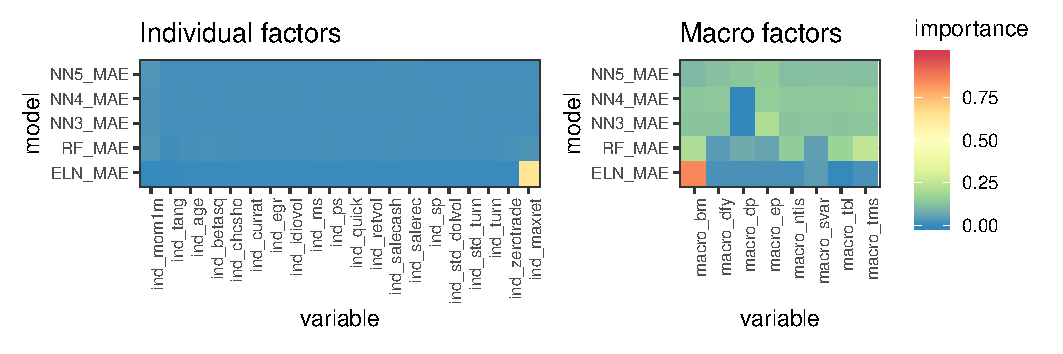
\includegraphics[max size = {\textwidth}{0.35\textheight}]{../../Results/empirical/empirical_all_sample_vi.pdf}
	\caption{Empirical individual and macroeconomic factor importance, averaged over all samples}
	\floatfoot{Individual factors shown on x axis (see Table \ref{ind_factors} in Appendix for definitions)}
\end{figure}

The elastic net, random forest and to a lesser extent DFNs tend to pick out the max return and 1 month momentum factors out of the individual characteristics as important, and the book-to-market factor out of the macroeconomic factors are important. In general, the variable importance metrics are less consistent for the random forests, and it should be noted in particular that the random forest tends to determine factors highly correlated with momentum as important, such as change in momentum, dollar trading volume and return volatility. Within the macroeconomic factors, penalized linear models tend to identify the average book to market ratio and the default spread as the most important. The random forests were inconsistent with the elastic nets, and tended to assign very similar variable importance metrics to most macroeconomic factors.

Interestingly, the linear models assign the controversial dividend price ratio macroeconomic factor as highly important, a result mirrored only with the neural networks. Their variable importance for individual factors across different training samples is non-robust, with the important variables almost completely changing year to year. The linear models consistently identified the controversial dividend-price ratio as important, a result that was somewhat consistent with the neural networks. 

The overall results again contradict the results of \cite{gu_empirical_2018}, who conclude that all of the machine methods agree on the same subset of important factors. Indeed, we only see mild consistency in variable importance between the elastic nets and random forests on the individual factors only - all other variable importance metrics were either inconsistent between different models, or non-robust.

%All models considered typically preferred sparse parameterizations. That is, most if not all of the individual factors had little to no importance across all models.\footnote{Note that because the variable importance here was not evaluated explicitly for each pairwise interaction term, some of the individual factors appear as slightly important. This is because setting an individual factor to zero also sets some of the macroeconomic pairwise terms to zero, increasing its apparent importance.}

\section{Conclusion}

Our findings demonstrate that the field of machine learning may offer certain tools to improve stock prediction and identification of true underlying factors. Penalized linear models and to a lesser extent, random forests are the best performing methods in the analysis undertaken.

Importantly, we find that DFNs fail in the context of stock return prediction, at both prediction performance and variable importance analysis. This result is consistent across a variety of simulated datasets, as well as empirical data. 

Lastly, we find that the top performing models - the elastic nets and random forests, tend to agree and correctly identify the correct underlying regressors in simulated contexts, and agree on the same subset of factors which are important in empirical contexts. We find that of all the models considered, the elastic nets are the most consistent at identifying true underlying regressors through the simulation study. We find that in the empirical setting, among the individual factors the 1 and 6 month momentum factors are the most powerful predictors of stock returns, according to the penalized linear models and random forests. 

The overall findings of this paper differ from the sparse literature on machine learning methods in empirical finance. However, the performance of the penalized linear models with respect to both out of sample prediction performance and variable importance analysis is promising, and our findings show that machine learning provides some tools which may aid in the problems of stock return prediction and risk factor selection in the financial world. 

\newpage

\subsection{Retrieval of style files}

The style files for NeurIPS and other conference information are available on
the World Wide Web at
\begin{center}
  \url{http://www.neurips.cc/}
\end{center}
The file \verb+neurips_2020.pdf+ contains these instructions and illustrates the
various formatting requirements your NeurIPS paper must satisfy.

The only supported style file for NeurIPS 2020 is \verb+neurips_2020.sty+,
rewritten for \LaTeXe{}.  \textbf{Previous style files for \LaTeX{} 2.09,
  Microsoft Word, and RTF are no longer supported!}

The \LaTeX{} style file contains three optional arguments: \verb+final+, which
creates a camera-ready copy, \verb+preprint+, which creates a preprint for
submission to, e.g., arXiv, and \verb+nonatbib+, which will not load the
\verb+natbib+ package for you in case of package clash.

\paragraph{Preprint option}
If you wish to post a preprint of your work online, e.g., on arXiv, using the
NeurIPS style, please use the \verb+preprint+ option. This will create a
nonanonymized version of your work with the text ``Preprint. Work in progress.''
in the footer. This version may be distributed as you see fit. Please \textbf{do
  not} use the \verb+final+ option, which should \textbf{only} be used for
papers accepted to NeurIPS.

At submission time, please omit the \verb+final+ and \verb+preprint+
options. This will anonymize your submission and add line numbers to aid
review. Please do \emph{not} refer to these line numbers in your paper as they
will be removed during generation of camera-ready copies.

The file \verb+neurips_2020.tex+ may be used as a ``shell'' for writing your
paper. All you have to do is replace the author, title, abstract, and text of
the paper with your own.

The formatting instructions contained in these style files are summarized in
Sections \ref{gen_inst}, \ref{headings}, and \ref{others} below.

\section{General formatting instructions}
\label{gen_inst}

The text must be confined within a rectangle 5.5~inches (33~picas) wide and
9~inches (54~picas) long. The left margin is 1.5~inch (9~picas).  Use 10~point
type with a vertical spacing (leading) of 11~points.  Times New Roman is the
preferred typeface throughout, and will be selected for you by default.
Paragraphs are separated by \nicefrac{1}{2}~line space (5.5 points), with no
indentation.

The paper title should be 17~point, initial caps/lower case, bold, centered
between two horizontal rules. The top rule should be 4~points thick and the
bottom rule should be 1~point thick. Allow \nicefrac{1}{4}~inch space above and
below the title to rules. All pages should start at 1~inch (6~picas) from the
top of the page.

For the final version, authors' names are set in boldface, and each name is
centered above the corresponding address. The lead author's name is to be listed
first (left-most), and the co-authors' names (if different address) are set to
follow. If there is only one co-author, list both author and co-author side by
side.

Please pay special attention to the instructions in Section \ref{others}
regarding figures, tables, acknowledgments, and references.

\section{Headings: first level}
\label{headings}

All headings should be lower case (except for first word and proper nouns),
flush left, and bold.

First-level headings should be in 12-point type.

\subsection{Headings: second level}

Second-level headings should be in 10-point type.

\subsubsection{Headings: third level}

Third-level headings should be in 10-point type.

\paragraph{Paragraphs}

There is also a \verb+\paragraph+ command available, which sets the heading in
bold, flush left, and inline with the text, with the heading followed by 1\,em
of space.

\section{Citations, figures, tables, references}
\label{others}

These instructions apply to everyone.

\subsection{Citations within the text}

The \verb+natbib+ package will be loaded for you by default.  Citations may be
author/year or numeric, as long as you maintain internal consistency.  As to the
format of the references themselves, any style is acceptable as long as it is
used consistently.

The documentation for \verb+natbib+ may be found at
\begin{center}
  \url{http://mirrors.ctan.org/macros/latex/contrib/natbib/natnotes.pdf}
\end{center}
Of note is the command \verb+\citet+, which produces citations appropriate for
use in inline text.  For example,
\begin{verbatim}
   \citet{hasselmo} investigated\dots
\end{verbatim}
produces
\begin{quote}
  Hasselmo, et al.\ (1995) investigated\dots
\end{quote}

If you wish to load the \verb+natbib+ package with options, you may add the
following before loading the \verb+neurips_2020+ package:
\begin{verbatim}
   \PassOptionsToPackage{options}{natbib}
\end{verbatim}

If \verb+natbib+ clashes with another package you load, you can add the optional
argument \verb+nonatbib+ when loading the style file:
\begin{verbatim}
   \usepackage[nonatbib]{neurips_2020}
\end{verbatim}

As submission is double blind, refer to your own published work in the third
person. That is, use ``In the previous work of Jones et al.\ [4],'' not ``In our
previous work [4].'' If you cite your other papers that are not widely available
(e.g., a journal paper under review), use anonymous author names in the
citation, e.g., an author of the form ``A.\ Anonymous.''

\subsection{Footnotes}

Footnotes should be used sparingly.  If you do require a footnote, indicate
footnotes with a number\footnote{Sample of the first footnote.} in the
text. Place the footnotes at the bottom of the page on which they appear.
Precede the footnote with a horizontal rule of 2~inches (12~picas).

Note that footnotes are properly typeset \emph{after} punctuation
marks.\footnote{As in this example.}

\subsection{Figures}

\begin{figure}
  \centering
  \fbox{\rule[-.5cm]{0cm}{4cm} \rule[-.5cm]{4cm}{0cm}}
  \caption{Sample figure caption.}
\end{figure}

All artwork must be neat, clean, and legible. Lines should be dark enough for
purposes of reproduction. The figure number and caption always appear after the
figure. Place one line space before the figure caption and one line space after
the figure. The figure caption should be lower case (except for first word and
proper nouns); figures are numbered consecutively.

You may use color figures.  However, it is best for the figure captions and the
paper body to be legible if the paper is printed in either black/white or in
color.

\subsection{Tables}

All tables must be centered, neat, clean and legible.  The table number and
title always appear before the table.  See Table~\ref{sample-table}.

Place one line space before the table title, one line space after the
table title, and one line space after the table. The table title must
be lower case (except for first word and proper nouns); tables are
numbered consecutively.

Note that publication-quality tables \emph{do not contain vertical rules.} We
strongly suggest the use of the \verb+booktabs+ package, which allows for
typesetting high-quality, professional tables:
\begin{center}
  \url{https://www.ctan.org/pkg/booktabs}
\end{center}
This package was used to typeset Table~\ref{sample-table}.

\begin{table}
  \caption{Sample table title}
  \label{sample-table}
  \centering
  \begin{tabular}{lll}
    \toprule
    \multicolumn{2}{c}{Part}                   \\
    \cmidrule(r){1-2}
    Name     & Description     & Size ($\mu$m) \\
    \midrule
    Dendrite & Input terminal  & $\sim$100     \\
    Axon     & Output terminal & $\sim$10      \\
    Soma     & Cell body       & up to $10^6$  \\
    \bottomrule
  \end{tabular}
\end{table}

\section{Final instructions}

Do not change any aspects of the formatting parameters in the style files.  In
particular, do not modify the width or length of the rectangle the text should
fit into, and do not change font sizes (except perhaps in the
\textbf{References} section; see below). Please note that pages should be
numbered.

\section{Preparing PDF files}

Please prepare submission files with paper size ``US Letter,'' and not, for
example, ``A4.''

Fonts were the main cause of problems in the past years. Your PDF file must only
contain Type 1 or Embedded TrueType fonts. Here are a few instructions to
achieve this.

\begin{itemize}

\item You should directly generate PDF files using \verb+pdflatex+.

\item You can check which fonts a PDF files uses.  In Acrobat Reader, select the
  menu Files$>$Document Properties$>$Fonts and select Show All Fonts. You can
  also use the program \verb+pdffonts+ which comes with \verb+xpdf+ and is
  available out-of-the-box on most Linux machines.

\item The IEEE has recommendations for generating PDF files whose fonts are also
  acceptable for NeurIPS. Please see
  \url{http://www.emfield.org/icuwb2010/downloads/IEEE-PDF-SpecV32.pdf}

\item \verb+xfig+ "patterned" shapes are implemented with bitmap fonts.  Use
  "solid" shapes instead.

\item The \verb+\bbold+ package almost always uses bitmap fonts.  You should use
  the equivalent AMS Fonts:
\begin{verbatim}
   \usepackage{amsfonts}
\end{verbatim}
followed by, e.g., \verb+\mathbb{R}+, \verb+\mathbb{N}+, or \verb+\mathbb{C}+
for $\mathbb{R}$, $\mathbb{N}$ or $\mathbb{C}$.  You can also use the following
workaround for reals, natural and complex:
\begin{verbatim}
   \newcommand{\RR}{I\!\!R} %real numbers
   \newcommand{\Nat}{I\!\!N} %natural numbers
   \newcommand{\CC}{I\!\!\!\!C} %complex numbers
\end{verbatim}
Note that \verb+amsfonts+ is automatically loaded by the \verb+amssymb+ package.

\end{itemize}

If your file contains type 3 fonts or non embedded TrueType fonts, we will ask
you to fix it.

\subsection{Margins in \LaTeX{}}

Most of the margin problems come from figures positioned by hand using
\verb+\special+ or other commands. We suggest using the command
\verb+\includegraphics+ from the \verb+graphicx+ package. Always specify the
figure width as a multiple of the line width as in the example below:
\begin{verbatim}
   \usepackage[pdftex]{graphicx} ...
   \includegraphics[width=0.8\linewidth]{myfile.pdf}
\end{verbatim}
See Section 4.4 in the graphics bundle documentation
(\url{http://mirrors.ctan.org/macros/latex/required/graphics/grfguide.pdf})

A number of width problems arise when \LaTeX{} cannot properly hyphenate a
line. Please give LaTeX hyphenation hints using the \verb+\-+ command when
necessary.


\section*{Broader Impact}

Authors are required to include a statement of the broader impact of their work, including its ethical aspects and future societal consequences. 
Authors should discuss both positive and negative outcomes, if any. For instance, authors should discuss a) 
who may benefit from this research, b) who may be put at disadvantage from this research, c) what are the consequences of failure of the system, and d) whether the task/method leverages
biases in the data. If authors believe this is not applicable to them, authors can simply state this.

Use unnumbered first level headings for this section, which should go at the end of the paper. {\bf Note that this section does not count towards the eight pages of content that are allowed.}

\begin{ack}
Use unnumbered first level headings for the acknowledgments. All acknowledgments
go at the end of the paper before the list of references. Moreover, you are required to declare 
funding (financial activities supporting the submitted work) and competing interests (related financial activities outside the submitted work). 
More information about this disclosure can be found at: \url{https://neurips.cc/Conferences/2020/PaperInformation/FundingDisclosure}.


Do {\bf not} include this section in the anonymized submission, only in the final paper. You can use the \texttt{ack} environment provided in the style file to autmoatically hide this section in the anonymized submission.
\end{ack}

\section*{References}

References follow the acknowledgments. Use unnumbered first-level heading for
the references. Any choice of citation style is acceptable as long as you are
consistent. It is permissible to reduce the font size to \verb+small+ (9 point)
when listing the references.
{\bf Note that the Reference section does not count towards the eight pages of content that are allowed.}
\medskip

\small

[1] Alexander, J.A.\ \& Mozer, M.C.\ (1995) Template-based algorithms for
connectionist rule extraction. In G.\ Tesauro, D.S.\ Touretzky and T.K.\ Leen
(eds.), {\it Advances in Neural Information Processing Systems 7},
pp.\ 609--616. Cambridge, MA: MIT Press.

[2] Bower, J.M.\ \& Beeman, D.\ (1995) {\it The Book of GENESIS: Exploring
  Realistic Neural Models with the General NEural SImulation System.}  New York:
TELOS/Springer--Verlag.

[3] Hasselmo, M.E., Schnell, E.\ \& Barkai, E.\ (1995) Dynamics of learning and
recall at excitatory recurrent synapses and cholinergic modulation in rat
hippocampal region CA3. {\it Journal of Neuroscience} {\bf 15}(7):5249-5262.


\appendix

\newpage

\section{Additional details: models}
In this section, we give a brief overview of all the models considered in the simulation and empirical study.

\subsection{Linear models}
Linear models model the conditional expectation \( g^*(z_{i, t}) \) as a linear function of the predictors and the parameter vector \( \theta \):
\begin{equation}
g(z_{i, t};\theta) = z_{i, t}' \theta
\end{equation}
This yields the OLS estimator when optimized w.r.t. MSE, and the LAD estimator when optimized w.r.t. MAE.

\subsection{Elastic nets}
Elastic Nets are similar to linear models but differ via the addition of a penalty term in the loss function:
\begin{equation}
\mathcal{L(\theta;.)} = 
\underset{\text{Loss Function}}{\underbrace{\mathcal{L(\theta)}}} + 
\underset{\text{Penalty Term}}{\underbrace{\phi(\theta;.)}}
\end{equation}
where the elastic net penalty \cite{zou_regularization_2005} is:
\begin{equation}
\phi(\theta;\lambda,\rho) = 
\lambda(1-\rho) \sum_{j = 1}^{P}|\theta_j| +
\frac{1}{2} \lambda \rho \sum_{j = 1}^{P}\theta_j^2
\end{equation}
where the hyperparameter $\lambda$ controls the overall magnitude of the loss, and hyperparameter $\rho$ controls the shape of the penalization. $\rho = 1$ corresponds to ridge regression proposed by \cite{hoerl_ridge_1970}, which uses $l_2$ penalty that shrinks all coefficients closer to 0, but not to 0. $\rho = 0$ case corresponds to the popular LASSO and uses absolute ($l_1$) parameter penalization proposed by \cite{tibshirani_regression_1996}, which geometrically allows the coefficients to be shrunk to 0. For \(0 < \rho < 1\), the elastic net aims to produce parsimonious models through both shrinkage and selection by combining the properties of LASSO and ridge regression.

\subsection{Random forests}
%% Explain CART first

Random Forests are an extension of Classification and Regression Trees (CART) proposed by \cite{breiman_random_2001}. CART are fully non-parametric models that can capture complex multi-way interactions. A tree "grows" in a series of iterations. With each iteration, a split ("branch") is made along one predictor such that it is the best split available at that stage with respect to minimizing the loss function. These steps are continued until each observation is its own node, or more commonly until the stopping criterion is met. The eventual model slices the predictor space into rectangular partitions, and predicts the unknown function $g^*(z_{i,t})$ with the average value of the outcome variable in each partition. The prediction of a tree, $\mathcal{T}$, with \(K\) "leaves" (terminal nodes), and depth $L$ is
\begin{equation}
g(z_{i,t};\theta,K,L) = \sum_{k=1}^{K}\theta_k\textbf{1}_{z_{i,t}\in C_k(L)}
\end{equation}
where $C_k(L)$ is one of the $K$ partitions in the model. For this study, only recursive binary trees were considered. Though trees were originally proposed and fit with respect to minimizing MSE, they can be grown with respect to a variety of loss functions, including MAE, where the loss within each C partition is denoted by $H(\theta, C)$: 
\begin{equation}
H(\theta, C) = \frac{1}{|C|} \sum_{z_{i,t} \in C} L(r_{i,t+1} - \theta)
\end{equation} 
where $|C|$ denotes the number of observations in set C (partition). Given $C$, it is clear that the optimal choice for minimising MSE is simply $\theta = \frac{1}{|C|} \sum_{z_{io,t}\in C}^{ }r_{i,t+1}$ i.e. the average of the partition, and the median of the partition when minimising MAE.

Trees, grown to a deep enough level, are highly unbiased and flexible, as each partition can potentially predict a single, or low number of observations. The trade-off is their high variance and instability. 

Further details are given in cite().

\subsection{Feed forward neural networks}
More specifically, a neural network consists of layers denoted by $l = 0, 1, \dots, L$, with $l = 0$ denoting the input layer and $l = L$ denoting the output layer. The input layer is defined by the scaled predictor set, $x^{(0)} = (1, z_1, \dots, z_N)'$. The model adds complexity through the use of one or more hidden layer, each containing $K^{(l)}$ "neurons". Each neuron linearly aggregates the values of the previous layer, and applies some non-linear "activation function" which we denote as $\alpha$ to its aggregated signal before sending its output to the next layer. The output of neuron $k$ in layer $l$ is then $x_k^{(l)}$. Next, define the vector of outputs for this layer as $x^{(l)} = (1, x_1^{(l)}, \dots, x_{K^(l)}^{(l)})'$.  The recursive output formula for the neural network at each neuron in layer $l > 0$ is then:
\begin{equation}
x_k^{(l)} = \alpha(x^{(l-1)'}\theta_k^{l-1}),
\end{equation}
where $\alpha()$ represents the activation function for that layer with the final output \footnote{Note that the specification of a constant ``1" at the beginning of each layer is the same as specifying a bias term as is popular in other parametrizations. }
\begin{equation}
g(z;\theta) = x^{(L-1)'}\theta^{L-1}
\end{equation}
The neural network's weight and bias parameters for each layer are estimated by minimizing the loss function with respect to the parameters, i.e. by calculating the partial derivative with respect to a specific weight or bias element. 

Due to the complexity and hence non-existent analytical form for this solution, this is typically found via backpropagation, an algorithm which exploits the chain rule of the partial derivative and iteratively finds a local optimum using a first order gradient based algorithm, also known as "gradient descent." The gradient descent algorithm minimizes some function (such as the loss function in the context of machine learning) by iteratively moving in the direction of steepest descent, defined as the negative gradient. Formally, for a loss function $L(x)$ that is defined and has a gradient defined in the neighbourhood of the parameter set $a$, the updating algorithm is:
\begin{equation}
a_{n+1} = a_n - \gamma \Delta F(a_n)
\end{equation}
where $\gamma$ controls the size of each update. This $\gamma$ parameter is known as the learning rate in neural network training, and controlling this is critical for good performance. As the loss functions of neural networks can be very complex with many local minima, the learning rate should be high enough such that the parameter updates are large enough to skip or jump over them. Too large of a learning rate however, and the neural may fail to converge to a solution at all. Due to computational limitations, we tune the learning rate manually, and consider a variety of different ``optimizers", or algorithms which adapt the learning rate in different ways (see Appendix for computational details).

For our application, we considered the following grid of hyperparameters:

Further details are given in cite().

\subsection{Long short term memory networks}
Long short term memory (LSTM) networks are 

For our application, we considered the following grid of hyperparameters:

\begin{itemize}
	\item 
\end{itemize}

Further details are given in cite().

\subsection{FFORMA}
Feature-based Forecast Model Averaging, cite() is an automated method for obtaining weighted forecast combinations for time series. We provide a brief overview of the two phases in this methodology.

Phase one involves training the meta learning model. Let $\mathbf{y_1}, \mathbf{y_2}, \dots, \mathbf{y_N}$ denote the different times series of excess returns, $F$ denote the set of functions for calculating time series features, and $M$ the set of constituent models considered for each times series. For each time series $\mathbf{y_n}$, split $\mathbf{y_n}$ into training, validation and test sets, calculate the set of features $f_n \in F$ over the training period, fit each constituent model $m \in M$ over the training period and generate forecasts over the validation and test periods, and calculate validation losses $L_{nm}$. Finally, train the meta-learning model by minimizing:
\begin{equation}
\underset{w}{\text{argmin}} \sum_{n = 1}^{N} \sum_{m = 1}^{M} w(f_n)_m L_{nm}
\end{equation}

To incorporate all regressors in each individual time series model, we applied dimensional reduction techniques of PCA and UMAP to generate new feature mappings for use in GARCH (1, 1) models (generally the best performing of the constituent models). None of the new external regressors as generated by these feature mappings improved performance, however.

The constituent models we considered are:
\begin{itemize}
	\item Naive
	\item Random walk with drift
	\item Theta method
	\item ARIMA
	\item ETS
	\item TBATS
	\item Neural network auto-regressive model
	\item ARMA (1, 1) with g.e.d. GARCH(1, 1) errors
	\item ARMA (1, 1) with g.e.d. GARCH(1, 1) errors and UMAP external regressors
\end{itemize}
We follow cite()'s selection of time series features as inputs to the meta-learner. The time series features used to train the meta-model are detailed in cite(), with the addition of realized volatility. Note that because financial returns data does not typically exhibit seasonality, features and constituent models related which utilized seasonality were omitted.

Phase two uses the learning model from phase one to produce new, combined forecasts for each time series. For each $\mathbf{y_n}$, calculate the features $f_{new}$ by applying $F$, use the meta-learner to produce $w(f_{new})$ an $M$ vector of weights, compute the forecasts from each constituent model in $M$, then finally combine them into a final forecast using weights $w$.

\subsection{DeepAR}
DeepAR is a generalization of traditional Auto Regressive (AR) models to include additional layers into order to introduce non-linearities into the model.

%% This is directly plonked from deepar arxiv paper, change this so this isn't plagiarism!
%% DeepAR does not require inputs from the entire cross section to produce forecasts!

DeepAR aims to model the conditional distribution of the 
\begin{equation*}
P(\zVec{i}{t_0}{T} | \zVec{i}{1}{t_0-1}, \xVec{i}{1}{T})
\label{eq:condDist}
\end{equation*}
of the future of each time series $[\z{i}{t_0}, \z{i}{t_0 + 1}, \ldots, \z{i}{T}] := \zVec{i}{t_0}{T}$ given its \hbox{past $[\z{i}{1}, \ldots, \z{i}{t_0-2}, \z{i}{t_0-1}] := \zVec{i}{1}{t_0-1}$}, where $t_0$ denotes the time point from which we assume $\z{i}{t}$ to be unknown at prediction time, and $\xVec{i}{1}{T}$ are covariates that are assumed to be known for all time points. To prevent confusion we avoid the ambiguous terms ``past'' and ``future'' and will refer to time ranges $[1, t_0-1]$ and $[t_0, T]$ as the conditioning range and 
prediction range, respectively. During training, both ranges have to lie in the past so that the $\z{i}{t}$ are observed, but during prediction $\z{i}{t}$ is only available in the conditioning range. Note that the time index $t$ is relative, i.e.\ $t=1$ can correspond to a different actual time period for each $i$. 

\newcommand{\modelDist}{Q_\Theta(\zVec{i}{t_0}{T} | \zVec{i}{1}{t_0-1}, \xVec{i}{1}{T})}

Our model, summarized in Fig.~\ref{fig:encoderdecoder}, is based on an autoregressive recurrent network architecture \cite{graves2013,sutskever2014}.
We assume that our model distribution $\modelDist$ consists of a product of likelihood factors
\begin{align*}
\modelDist &= \prod\nolimits_{t=t_0}^T Q_\Theta(z_{i,t}|\mathbf{z}_{i,1:t-1}, \xVec{i}{1}{T}) = \prod\nolimits_{t=t_0}^T \ell(\z{i}{t} | \theta(\hVec_{i, t}, \Theta))
\end{align*}
parametrized by the output $\hVec_{i, t}$ of an autoregressive recurrent network
\begin{equation}
\hVec_{i, t} = h\left(\hVec_{i, t-1}, \z{i}{t-1}, \xbf_{i, t}, \Theta\right) \,,
\label{eq:recurrence}
\end{equation}
where $h$ is a function implemented by a multi-layer recurrent neural network with LSTM cells.% 
\footnote{Details of the architecture and hyper-parameters are given in the supplementary material.}
The model is autoregressive, in the sense that it consumes the observation at the last time step $\z{i}{t-1}$ as an input,
as well as recurrent, i.e.\ the previous output of the network $\hVec_{i,t-1}$ is fed back as an input at the next time step.
The likelihood $\ell(\z{i}{t}|\theta(\hVec_{i,t}))$ is a fixed distribution
whose parameters are given by a function $\theta(\hVec_{i,t}, \Theta)$ of the network output $\hVec_{i, t}$ (see below).

Information about the observations in the conditioning range $\zVec{i}{1}{t_0 -1}$ is transferred to the prediction range through the initial state $\hVec_{i, t_0-1}$. In the sequence-to-sequence setup, this initial state is the output of an \emph{encoder network}. While in general this encoder network can have a different architecture, in our 
experiments we opt for using the same architecture for the model in the conditioning range and the prediction range (corresponding to the \emph{encoder} and \emph{decoder} in
a sequence-to-sequence model). Further, we share weights between them, so that the initial state
for the decoder $\hVec_{i, t_0 - 1}$ is obtained by computing \eqref{eq:recurrence} for $t = 1, \ldots, t_0 - 1$, where all required quantities are observed. The initial state of the encoder $\hVec_{i, 0}$ as well as $\z{i}{0}$ are initialized to zero.

Given the model parameters $\Theta$, we can directly obtain joint samples $\tilde{\mathbf{z}}_{i, t_0:T} \sim \modelDist$ through ancestral sampling:
First, we obtain $\hVec_{i, t_0-1}$ by computing \eqref{eq:recurrence} for $t=1,\ldots, t_0$.
For $t=t_0, t_0+1, \ldots, T$ we sample $\tilde{z}_{i, t} \sim \ell(\cdot | \theta(\tilde{\mathbf{h}}_{i,t}, \Theta))$
where $\tilde{\mathbf{h}}_{i, t} = h\left(\hVec_{i, t-1}, \tilde{z}_{i, t-1}, \xbf_{i, t}, \Theta\right)$
initialized with $\tilde{\mathbf{h}}_{i, t_0-1} = \hVec_{i, t_0-1}$ and $\tilde{z}_{i, t_0 -1} = \z{i}{t_0 - 1}$.
Samples from the model obtained in this way can then be used to compute quantities
of interest, e.g.\ quantiles of the distribution of the sum of values for some
time range in the future.

Further details are given in cite().

\appendix

\newpage

\section{Additional details: simulation design}
In this section, we give additional features of the simulation design required to implenent our results. All code and data can be found at XXXX. 

\subsection{Simulation Design}

We begin with the simulation study as a way to explore how machine learning performs with regards to the stylized facts of empirical returns in a controlled environment. We simulate according to a design which incorporates low signal to noise ratio, stochastic volatility in errors, persistence and cross sectional correlation in regressors. Our specification is a latent factor model for excess returns $r_{t+1}$, for $t=1, \dots, T$:
\begin{align}
r_{i, t+1} &= 
g\left(z_{i, t}\right) + \beta_{i,t+1}v_{t+1} + e_{i, t+1}; 
\enspace z_{i, t} = \left(1, x_{t}\right)^{\prime} \otimes c_{i, t}, 
\enspace \beta_{i, t} = \left(c_{i 1, t}, c_{i 2, t}, c_{i 3, t}\right) \\ 
e_{i, t+1} &= 
\sigma_{i, t+1} \varepsilon_{i, t+1}; \\
\operatorname{log} (\sigma^2_{i,t+1}) &= 
\omega + \gamma \operatorname{log} (\sigma^2_{t}) + \sigma_{u}u;
\quad u \sim N(0, 1)
\end{align}
where $v_{t+1}$ is a $3\times 1$ vector of errors, $w_{t+1} \sim N(0, 1)$,  $\varepsilon_{i,t+1} \sim N(0, 1)$ scalar error terms, matrix $C_t$ is an $N\times P_c$ matrix of latent factors, where the first three columns correspond to $\beta_{i,t}$, across the $1\leq i\leq N$ dimensions, while the remaining $P_c-3$ factors do not enter the return equation. The $P_x\times1$ vector $x_t$ is a $3 \times 1$ multivariate time series, and $\varepsilon_{t+1}$ is a $N\times 1$ vector of idiosyncratic errors. The parameters of these were tuned such that the annualized volatility of each return series was approximately 22\%, as is often observed empirically.
%%%%%%%%%%%%%%%%%%%%%
\paragraph{Simulating characteristics}
We build in correlation across time among factors by drawing normal random numbers for each $1\leq i\leq N$ and $1\leq j\leq P_{c}$, according to :
\begin{equation}
\overline{c}_{i j, t} = \rho_{j} \overline{c}_{i j, t-1}+\epsilon_{i j, t} ;
\quad \rho_{j} \sim \mathcal{U} \left( 0.5, 1 \right) 
\end{equation}
We then build in cross sectional correlation:
\begin{align}
\widehat{C}_{t}&=L\overline{C}_{t} ; \quad B = LL' \\
B:&=\Lambda\Lambda' + 0.1\mathbb{I}_{n}, \quad
\Lambda_i = (\lambda_{i1}, \dots, \lambda_{i4}), \quad
\lambda_{ik}\sim N(0, \lambda_{sd}), \; k=1, \dots, 4
\end{align}
where $B$ serves as a variance covariance matrix with $\lambda_{sd}$ its density, and $L$ represents the lower triangle matrix of $B$ via the Cholesky decomposition. $\lambda_{sd}$ values of 0.01, 0.1 and 1 were used to explore increasing degrees of cross sectional correlation.
Characteristics are then normalized to be within $[-1, 1]$ for each $1\leq i\leq N$ and for $j=1, \dots, P_{c}$ via:
\begin{equation}
c_{i j, t} = \frac{2}{n+1} \operatorname{rank}\left(\hat{c}_{i j, t}\right) - 1.
\end{equation}
%%%%%%%%%%%%%%%%%%%%%%
\paragraph{Simulating macroeconomic series}
We consider a Vector Autoregression (VAR) model for $x_{t}$, a $3 \times 1$ multivariate time series \footnote{More complex specifications for $A$ were briefly explored, but these did not have a significant impact on results.}:
\begin{flalign*}
x_{t} = Ax_{t-1}+u_t; 
\quad A = 0.95 I_3;
\quad u_t \sim N\left( \mu = (0, 0, 0)' , \Sigma = I_3
\right) 
\end{flalign*}
\paragraph{Simulating return series}
We consider three different functions for $g(z_{i, t})$:
\begin{align}
(1)\; & g_1 \left(z_{i, t}\right)=\left(c_{i 1, t}, c_{i 2, t}, c_{i 3, t} \times x_{t}'[3,]\right) \theta_{0} \\
(2)\; & g_2 \left(z_{i, t}\right)=\left(c_{i 1, t}^{2}, c_{i 1, t} \times c_{i 2, t}, \operatorname{sgn}\left(c_{i 3, t} \times  x_{t}'[3,]\right)\right) \theta_{0} \\
(3)\; & g_3 \left(z_{i, t}\right) = \left(1[c_{i3,t}>0],c_{i 2, t}^{3}, c_{i 1, t} \times c_{i 2, t}\times 1[c_{i3,t}>0], \text{logit}\left({c}_{i3, t} \right)\right) \theta_{0}
\end{align}
where $x_{t}'[3,]$ denotes the third element of the $x_{t}'$ vector.
%%%%%%%%%%%%%%%%%%%%%%%%%
$g_1 \left(z_{i, t}\right)$ allows the characteristics to enter the return equation linearly, and $g_2 \left(z_{i, t}\right)$ and $g_3 \left(z_{i, t}\right)$ allow the characteristics to enter the return equation interactively and non-linearly. \footnote{($g_1, g_2$ correspond to the simulation design used by \cite{gu_empirical_2018}.)} $\theta^0$ was tuned such that the predictive $R^2$ was approximately 5\%.

The simulation design results in $3 \times 3 = 9$ different simulated datasets, each with $N = 200$ stocks, $T = 180$ periods and $P_c = 100$ characteristics. Each design was simulated 10 times to assess the robustness of machine learning algorithms, with the number of simulations kept low for computational feasibility. We employ the hybrid data splitting approach with a training:validation length ratio of approximately 1.5 and a test set that is 1 year in length. 

\subsubsection{Sample Splitting}

If viewed as monthly periods, $T = 180$ corresponds to 15 years. A data splitting scheme similar to the scheme to be used in the empirical data study was used: a training:validation length ratio of approximately 1.5 to begin, and a test set that is 1 year in length. We employ the hybrid growing window approach as described earlier in section \ref{sample_split} (see Figure \ref{sample_split_diag} for a graphical representation).

\begin{figure}[!htb]
	\begin{center}
		\begin{tabular}{|c|p{0.30cm}p{0.30cm}p{0.30cm}p{0.30cm}p{0.30cm}p{0.30cm}p{0.30cm}p{0.30cm}p{0.30cm}p{0.30cm}p{0.30cm}p{0.30cm}p{0.30cm}p{0.30cm}p{0.30cm}|}
			\hline
			Set No. &&&&&&&&&&&&&&& \\
			\hline
			%%%%%%%%
			3 & \cellcolor{cyan} & \cellcolor{cyan} & \cellcolor{cyan} & \cellcolor{cyan} & \cellcolor{cyan} & \cellcolor{cyan} & \cellcolor{cyan} & \cellcolor{cyan} & \cellcolor{cyan} &
			\cellcolor{pink} & \cellcolor{pink} & \cellcolor{pink} & \cellcolor{pink} & \cellcolor{pink} & 	
			\cellcolor{olive} \\
			%%%%%%%%
			2 & \cellcolor{cyan} & \cellcolor{cyan} & \cellcolor{cyan} & \cellcolor{cyan} & \cellcolor{cyan} & \cellcolor{cyan} & \cellcolor{cyan} & \cellcolor{cyan} &
			\cellcolor{pink} & \cellcolor{pink} & \cellcolor{pink} & \cellcolor{pink} & \cellcolor{pink} & 	
			\cellcolor{olive} & NA  \\
			%%%%%%%%
			1 & \cellcolor{cyan} & \cellcolor{cyan} & \cellcolor{cyan} & \cellcolor{cyan} & \cellcolor{cyan} & \cellcolor{cyan} & \cellcolor{cyan} &
			\cellcolor{pink} & \cellcolor{pink} & \cellcolor{pink} & \cellcolor{pink} & \cellcolor{pink} & 	
			\cellcolor{olive} & NA & NA \\
			\hline
			Year & 1 & 2 & 3 & 4 & 5 & 6 & 7 & 8 & 9 & 10 & 11 & 12 & 13 & 14 & 15\\
			\hline
		\end{tabular}
		\medskip
		\begin{tabular}{|c|p{0.30cm}|}
			\hline
			Training & \cellcolor{cyan} \\
			\hline
			Validation & \cellcolor{pink} \\
			\hline
			Test & \cellcolor{olive} \\
			\hline
		\end{tabular}
	\end{center}
	\caption{Sample Splitting Procedure}
	\label{sample_split_diag}
\end{figure}

Other schemes in the forecasting literature such as using an ``inner" rolling window validation loop to find the best hyperparameters on average, finally aggregating them in an ``outer" loop for a more robust error were considered but not implemented due to a) computational feasibility and b) the relative instability of optimal hyperparameters across different different windows.

\newpage

%%%%%%%%%%%%%%%%%%%%%%%%%%%%%%%%%%%%%%%%%%%%%%%%%%%%%%%%%%%%%%%%%%%%%%%%%%%%%%%%%%%%%%%%%%%%%%%
\subsection{Simulation Study Results}

\subsubsection{Prediction Performance}

%% Put in comprehensive tables here
%% May need to resize/re-generate this table so that it fits better
\begingroup\fontsize{6}{8}\selectfont

\begin{longtable}{ccccccccccc}
\toprule
\multicolumn{1}{c}{ } & \multicolumn{1}{c}{ } & \multicolumn{3}{c}{g1} & \multicolumn{3}{c}{g2} & \multicolumn{3}{c}{g3} \\
\cmidrule(l{3pt}r{3pt}){3-5} \cmidrule(l{3pt}r{3pt}){6-8} \cmidrule(l{3pt}r{3pt}){9-11}
model & Corr & Test MAE & Test MSE & Test $R^2$ & Test MAE & Test MSE & Test $R^2$ & Test MAE & Test MSE & Test $R^2$\\
\midrule
\endfirsthead
\multicolumn{11}{@{}l}{}\\
\toprule
\multicolumn{1}{c}{ } & \multicolumn{1}{c}{ } & \multicolumn{3}{c}{g1} & \multicolumn{3}{c}{g2} & \multicolumn{3}{c}{g3} \\
\cmidrule(l{3pt}r{3pt}){3-5} \cmidrule(l{3pt}r{3pt}){6-8} \cmidrule(l{3pt}r{3pt}){9-11}
model & Corr & Test MAE & Test MSE & Test $R^2$ & Test MAE & Test MSE & Test $R^2$ & Test MAE & Test MSE & Test $R^2$\\
\midrule
\endhead
\
\endfoot
\bottomrule
\endlastfoot
 & 0.01 & 0.036678 & 0.002740 & 0.008273 & 0.038255 & 0.002880 & -0.111788 & 0.037310 & 0.002795 & -0.032068\\
\cmidrule{2-11}
 & 0.10 & 0.036965 & 0.002765 & -0.011020 & 0.038580 & 0.002914 & -0.142944 & 0.037569 & 0.002817 & -0.054940\\
\cmidrule{2-11}
\multirow{-3}{*}{\centering\arraybackslash LM.MSE} & 1.00 & 0.042949 & 0.003414 & -0.438797 & 0.045376 & 0.003717 & -0.780953 & 0.043434 & 0.003469 & -0.488779\\
\cmidrule{1-11}
 & 0.01 & 0.036642 & 0.002737 & 0.009050 & 0.038348 & 0.002886 & -0.116369 & 0.037324 & 0.002797 & -0.035162\\
\cmidrule{2-11}
 & 0.10 & 0.036811 & 0.002755 & 0.002919 & 0.038745 & 0.002927 & -0.152580 & 0.037489 & 0.002810 & -0.047675\\
\cmidrule{2-11}
\multirow{-3}{*}{\centering\arraybackslash LM.MAE} & 1.00 & 0.042340 & 0.003344 & -0.393044 & 0.045342 & 0.003685 & -0.769955 & 0.043535 & 0.003468 & -0.544524\\
\cmidrule{1-11}
 & 0.01 & 0.034588 & 0.002566 & 0.140335 & 0.036223 & 0.002690 & 0.036877 & 0.035353 & 0.002623 & 0.099142\\
\cmidrule{2-11}
 & 0.10 & 0.034563 & 0.002564 & 0.144238 & 0.036183 & 0.002686 & 0.037258 & 0.035292 & 0.002617 & 0.100241\\
\cmidrule{2-11}
\multirow{-3}{*}{\centering\arraybackslash ELN.MSE} & 1.00 & 0.034614 & 0.002568 & 0.167184 & 0.036276 & 0.002698 & 0.037839 & 0.035444 & 0.002630 & 0.119875\\
\cmidrule{1-11}
 & 0.01 & 0.034579 & 0.002565 & 0.140982 & 0.036195 & 0.002688 & 0.039169 & 0.035334 & 0.002621 & 0.100442\\
\cmidrule{2-11}
 & 0.10 & 0.034558 & 0.002564 & 0.144627 & 0.036173 & 0.002688 & 0.038875 & 0.035285 & 0.002617 & 0.100919\\
\cmidrule{2-11}
\multirow{-3}{*}{\centering\arraybackslash ELN.MAE} & 1.00 & 0.034599 & 0.002567 & 0.167771 & 0.036305 & 0.002703 & 0.036583 & 0.035465 & 0.002631 & 0.118022\\
\cmidrule{1-11}
 & 0.01 & 0.035775 & 0.002671 & 0.063426 & 0.035718 & 0.002657 & 0.067615 & 0.035803 & 0.002661 & 0.070298\\
\cmidrule{2-11}
 & 0.10 & 0.035769 & 0.002665 & 0.066738 & 0.035684 & 0.002652 & 0.069139 & 0.035867 & 0.002670 & 0.062839\\
\cmidrule{2-11}
\multirow{-3}{*}{\centering\arraybackslash RF.MSE} & 1.00 & 0.036233 & 0.002698 & 0.068774 & 0.035989 & 0.002683 & 0.057103 & 0.036213 & 0.002695 & 0.069887\\
\cmidrule{1-11}
 & 0.01 & 0.035459 & 0.002643 & 0.083338 & 0.035420 & 0.002630 & 0.087653 & 0.035540 & 0.002645 & 0.086529\\
\cmidrule{2-11}
 & 0.10 & 0.035515 & 0.002649 & 0.081425 & 0.035489 & 0.002634 & 0.083405 & 0.035569 & 0.002644 & 0.081643\\
\cmidrule{2-11}
\multirow{-3}{*}{\centering\arraybackslash RF.MAE} & 1.00 & 0.035916 & 0.002675 & 0.087081 & 0.035643 & 0.002644 & 0.080965 & 0.036053 & 0.002679 & 0.075357\\
\cmidrule{1-11}
 & 0.01 & 0.036452 & 0.002722 & 0.016344 & 0.036768 & 0.002732 & -0.003917 & 0.036687 & 0.002738 & 0.009335\\
\cmidrule{2-11}
 & 0.10 & 0.036462 & 0.002719 & 0.020422 & 0.036776 & 0.002734 & -0.007259 & 0.036733 & 0.002737 & 0.002955\\
\cmidrule{2-11}
\multirow{-3}{*}{\centering\arraybackslash NN1.MSE} & 1.00 & 0.037545 & 0.002821 & -0.014452 & 0.037049 & 0.002764 & -0.014697 & 0.037459 & 0.002798 & -0.012469\\
\cmidrule{1-11}
 & 0.01 & 0.035960 & 0.002679 & 0.055814 & 0.036921 & 0.002747 & -0.015105 & 0.036305 & 0.002700 & 0.039371\\
\cmidrule{2-11}
 & 0.10 & 0.036082 & 0.002687 & 0.050698 & 0.037010 & 0.002750 & -0.020562 & 0.036322 & 0.002702 & 0.032303\\
\cmidrule{2-11}
\multirow{-3}{*}{\centering\arraybackslash NN1.MAE} & 1.00 & 0.037889 & 0.002834 & -0.043182 & 0.037979 & 0.002845 & -0.084075 & 0.037306 & 0.002793 & 0.002178\\
\cmidrule{1-11}
 & 0.01 & 0.037019 & 0.002785 & -0.021787 & 0.037320 & 0.002775 & -0.043354 & 0.037089 & 0.002774 & -0.017304\\
\cmidrule{2-11}
 & 0.10 & 0.036977 & 0.002765 & -0.021276 & 0.037009 & 0.002748 & -0.027538 & 0.036990 & 0.002758 & -0.020645\\
\cmidrule{2-11}
\multirow{-3}{*}{\centering\arraybackslash NN2.MSE} & 1.00 & 0.037536 & 0.002814 & -0.013978 & 0.036903 & 0.002752 & -0.005866 & 0.037516 & 0.002809 & -0.016934\\
\cmidrule{1-11}
 & 0.01 & 0.035894 & 0.002672 & 0.057743 & 0.036834 & 0.002740 & -0.007158 & 0.036335 & 0.002703 & 0.036305\\
\cmidrule{2-11}
 & 0.10 & 0.035890 & 0.002668 & 0.060310 & 0.036937 & 0.002750 & -0.017077 & 0.036270 & 0.002696 & 0.037157\\
\cmidrule{2-11}
\multirow{-3}{*}{\centering\arraybackslash NN2.MAE} & 1.00 & 0.037480 & 0.002814 & -0.009529 & 0.037715 & 0.002823 & -0.065390 & 0.037471 & 0.002804 & -0.010118\\
\cmidrule{1-11}
 & 0.01 & 0.036783 & 0.002757 & -0.006762 & 0.036840 & 0.002738 & -0.007525 & 0.037036 & 0.002764 & -0.020078\\
\cmidrule{2-11}
 & 0.10 & 0.036938 & 0.002761 & -0.015399 & 0.036852 & 0.002738 & -0.015106 & 0.036874 & 0.002757 & -0.004406\\
\cmidrule{2-11}
\multirow{-3}{*}{\centering\arraybackslash NN3.MSE} & 1.00 & 0.037424 & 0.002808 & -0.012964 & 0.036938 & 0.002754 & -0.006353 & 0.037420 & 0.002799 & -0.010348\\
\cmidrule{1-11}
 & 0.01 & 0.035816 & 0.002670 & 0.065432 & 0.036934 & 0.002749 & -0.016398 & 0.036471 & 0.002718 & 0.029948\\
\cmidrule{2-11}
 & 0.10 & 0.035893 & 0.002677 & 0.062002 & 0.036859 & 0.002741 & -0.011850 & 0.036200 & 0.002693 & 0.040611\\
\cmidrule{2-11}
\multirow{-3}{*}{\centering\arraybackslash NN3.MAE} & 1.00 & 0.037009 & 0.002774 & 0.021329 & 0.037270 & 0.002783 & -0.029644 & 0.037413 & 0.002792 & -0.008307\\
\cmidrule{1-11}
 & 0.01 & 0.036881 & 0.002759 & -0.020620 & 0.036856 & 0.002742 & -0.007715 & 0.037126 & 0.002775 & -0.026563\\
\cmidrule{2-11}
 & 0.10 & 0.036877 & 0.002761 & -0.014579 & 0.037221 & 0.002762 & -0.048711 & 0.036872 & 0.002748 & -0.008894\\
\cmidrule{2-11}
\multirow{-3}{*}{\centering\arraybackslash NN4.MSE} & 1.00 & 0.037382 & 0.002805 & -0.006481 & 0.036897 & 0.002751 & -0.005369 & 0.037354 & 0.002797 & -0.007739\\
\cmidrule{1-11}
 & 0.01 & 0.035935 & 0.002678 & 0.057720 & 0.036897 & 0.002749 & -0.010917 & 0.036708 & 0.002738 & 0.007046\\
\cmidrule{2-11}
 & 0.10 & 0.035828 & 0.002665 & 0.065041 & 0.036933 & 0.002749 & -0.019112 & 0.036273 & 0.002695 & 0.037704\\
\cmidrule{2-11}
\multirow{-3}{*}{\centering\arraybackslash NN4.MAE} & 1.00 & 0.037095 & 0.002779 & 0.019866 & 0.037323 & 0.002795 & -0.029377 & 0.037301 & 0.002787 & -0.001888\\
\cmidrule{1-11}
 & 0.01 & 0.037231 & 0.002785 & -0.049970 & 0.036931 & 0.002747 & -0.017002 & 0.037114 & 0.002772 & -0.021895\\
\cmidrule{2-11}
 & 0.10 & 0.037026 & 0.002767 & -0.032190 & 0.037176 & 0.002762 & -0.039436 & 0.036909 & 0.002757 & -0.011352\\
\cmidrule{2-11}
\multirow{-3}{*}{\centering\arraybackslash NN5.MSE} & 1.00 & 0.037364 & 0.002795 & -0.010495 & 0.036928 & 0.002755 & -0.005376 & 0.037475 & 0.002807 & -0.014974\\
\cmidrule{1-11}
 & 0.01 & 0.035888 & 0.002669 & 0.058579 & 0.036835 & 0.002738 & -0.008646 & 0.036685 & 0.002737 & 0.004643\\
\cmidrule{2-11}
 & 0.10 & 0.036038 & 0.002680 & 0.050976 & 0.036745 & 0.002727 & -0.004935 & 0.036484 & 0.002710 & 0.018192\\
\cmidrule{2-11}
\multirow{-3}{*}{\centering\arraybackslash NN5.MAE} & 1.00 & 0.037285 & 0.002794 & 0.002541 & 0.037038 & 0.002765 & -0.012729 & 0.037193 & 0.002775 & 0.002572\\
\cmidrule{1-11}
 & 0.01 & 0.037296 & 0.002798 & -0.043289 & 0.037227 & 0.002776 & -0.044764 & 0.037591 & 0.002818 & -0.062516\\
\cmidrule{2-11}
 & 0.10 & 0.037237 & 0.002795 & -0.031955 & 0.037134 & 0.002767 & -0.038255 & 0.037198 & 0.002785 & -0.030394\\
\cmidrule{2-11}
\multirow{-3}{*}{\centering\arraybackslash LSTM.MSE} & 1.00 & 0.038128 & 0.002851 & -0.082027 & 0.037382 & 0.002792 & -0.044243 & 0.037780 & 0.002830 & -0.044330\\
\cmidrule{1-11}
 & 0.01 & 0.037431 & 0.002805 & -0.056406 & 0.037337 & 0.002780 & -0.051854 & 0.037627 & 0.002817 & -0.067433\\
\cmidrule{2-11}
 & 0.10 & 0.037446 & 0.002804 & -0.062952 & 0.037118 & 0.002768 & -0.032544 & 0.037241 & 0.002793 & -0.033320\\
\cmidrule{2-11}
\multirow{-3}{*}{\centering\arraybackslash LSTM.MAE} & 1.00 & 0.038027 & 0.002846 & -0.061483 & 0.037415 & 0.002790 & -0.045506 & 0.037743 & 0.002825 & -0.045884\\
\cmidrule{1-11}
 & 0.01 & 0.038277 & 0.002882 & -0.132672 & 0.038460 & 0.002889 & -0.147390 & 0.042466 & 0.003311 & -0.486145\\
\cmidrule{2-11}
 & 0.10 & 0.038358 & 0.002895 & -0.140765 & 0.038479 & 0.002891 & -0.160062 & 0.042323 & 0.003291 & -0.473991\\
\cmidrule{2-11}
\multirow{-3}{*}{\centering\arraybackslash FFORMA.MSE} & 1.00 & 0.038875 & 0.002965 & -0.131239 & 0.038808 & 0.002933 & -0.165990 & 0.043013 & 0.003371 & -0.470954\\
\cmidrule{1-11}
 & 0.01 & 0.038755 & 0.002939 & -0.179748 & 0.038747 & 0.002918 & -0.174094 & 0.042989 & 0.003365 & -0.527909\\
\cmidrule{2-11}
 & 0.10 & 0.038936 & 0.002951 & -0.192793 & 0.038796 & 0.002946 & -0.175994 & 0.043097 & 0.003406 & -0.586375\\
\cmidrule{2-11}
\multirow{-3}{*}{\centering\arraybackslash FFORMA.MAE} & 1.00 & 0.039247 & 0.002972 & -0.163656 & 0.039387 & 0.002996 & -0.211619 & 0.043709 & 0.003448 & -0.526081\\
\cmidrule{1-11}
 & 0.01 & 0.038299 & 0.002900 & -0.128930 & 0.038489 & 0.002912 & -0.132518 & 0.039390 & 0.003016 & -0.204980\\
\cmidrule{2-11}
 & 0.10 & 0.038832 & 0.002935 & -0.181663 & 0.038435 & 0.002905 & -0.131874 & 0.039177 & 0.002993 & -0.190558\\
\cmidrule{2-11}
\multirow{-3}{*}{\centering\arraybackslash DeepAR} & 1.00 & 0.040535 & 0.003159 & -0.239142 & 0.038787 & 0.002952 & -0.144029 & 0.039692 & 0.003042 & -0.182365\\*
\end{longtable}
\endgroup{}

\FloatBarrier

\subsection{Random Forest VIMPs}

We note that random forest methods typically have their own methodologies to calculate variable importance which are different to the variable importance metric presented in the main body of the paper. Here we provide two popular schemes of calculating random forest variable importance metrics - Breiman-cutler VIMP (traditional) and Ishwaran-Kogalur VIMP, and show that importantly, the overall conclusion regarding factor selection does not change with respect to which vimp methodology employed.

%% Re-generate or resize these graphs

\begin{figure}
	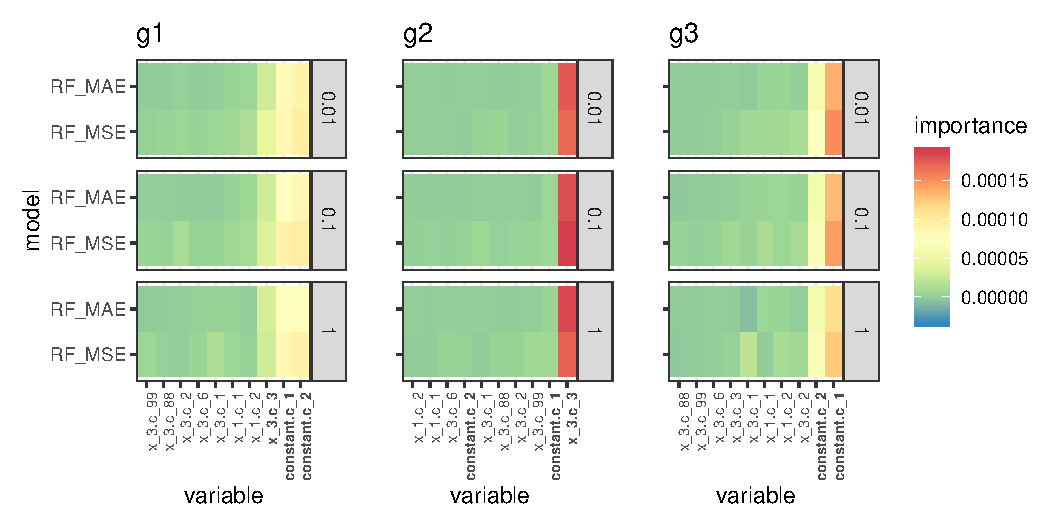
\includegraphics[max size = {\textwidth}{0.4\textheight}]{../../Results/simulation/graphics/simulation_g_vimp_bc.pdf}
	\caption{Simulation Breiman-Cutler vimps}
\end{figure}

%%IK

\begin{figure}
	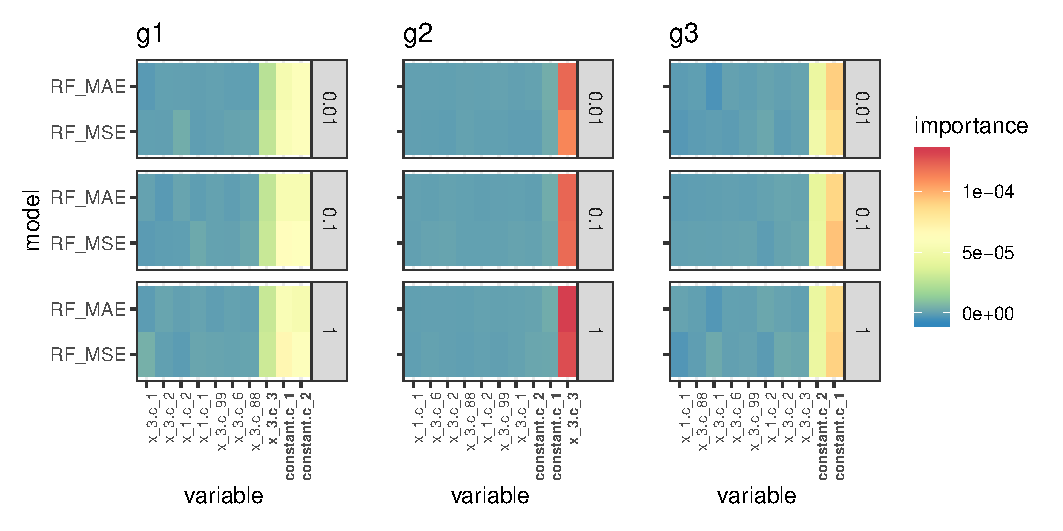
\includegraphics[max size = {\textwidth}{0.4\textheight}]{../../Results/simulation/graphics/simulation_g_vimp_ik.pdf}
	\caption{Simulation Ishwaran-Kogalur vimps}
\end{figure}

\newpage

\appendix

\section{Additional details: Empirical analysis}

\subsection{Data \& cleaning}

We begin by obtaining monthly individual price data from CRSP for all firms listed in the NYSE, AMEX and NASDAQ, starting from 1957 (starting date of the S\&P 500) and ending in December 2016, totalling 60 years. To build individual factors, we construct a factor set based on the cross section of returns literature. This data was sourced from and is the same data used in \cite{gu_empirical_2018}. Like our initial returns sample, it begins in March 1957 and ends in December 2016, totalling 60 years. It contains 94 stock level characteristics: 61 updated annually, 13 updated quarterly and 20 updated monthly, in addition to 74 industry dummies corresponding the the first two digits of the Standard Industrial Classification (SIC) codes. The dataset so far contains all securities traded, including those with a CRSP share code other than 10 or 11 and thus includes instruments such as REITs and mutual funds, and those with a share price of less than \$5.

% Begin Cleaning

To reduce the size of the dataset and increase feasibility, the dataset was filtered such that only stocks traded primarily on NASDAQ were included (using the PRIMEXCH variable from WRDS). Then, penny stocks (also referred to as microcaps in the literature) with a stock price of less than \$5 were filtered out, as is commonly done in the literature to reduce variability. Stocks without a share code of 10 or 11 (referring to equities) were filtered out, so that securities that are not equities were not included (such as REITs and trust funds). The monthly updated dataset was then converted to a quarterly format, to achieve a balance between having a dataset with enough data points and variability among factors. Quarterly returns were then constructed using the PRC variable according to actual returns:
\begin{equation}
RET_t = (PRC_t - PRC_{t-1})/PRC_{t-1}
\end{equation}
We allow all stocks which have a quarterly return to enter the dataset, even if they disappear from the dataset for certain periods, as opposed to only keeping stocks which appear continuously throughout the entire period. This was primarily done to reduce survivorship bias in the dataset, which can be very prevalent in financial data, and also allows for stocks which were unlisted and relisted again to feature in the dataset. 

The sic2 variable, corresponding to the stocks' Standard Industrial Classification (SIC) codes was dropped. The SIC code system suffers from inconsistent logic in classifying companies, and as a system built for pre-1970s traditional industries has been slow in recognizing new and emerging industries. Indeed, WRDS explicitly cautions the use of SIC codes beyond the use of rough grouping of industries, warning that SIC codes are not strictly enforced by government agencies for accuracy, in addition to most large companies belonging to multiple SIC codes over time. Because of this latter point in particular, there can be inconsistencies on the correct SIC code for the same company depending on the data source. Dropping the sic2 variable also reduced the dimensionality of the dataset by 74 columns, significantly increasing computational feasibility.

There existed a significant amount of missing data in the dataset. For the main empirical study, any characteristics that had over 20\% of their data were removed, and remaining missing data points were then imputed with their cross sectional medians. However, as the amount of missing data increases dramatically going further back in time, a balance between using more periods at the cost of removing more characteristics versus using less periods but keeping more characteristics was needed. 1993 Q3 was determined to be a reasonable time frame to begin the dataset due to a noticeable increase in data quality.

We then follow \cite{gu_empirical_2018} and construct eight macroeconomic factors following the variable definitions in \cite{welch_comprehensive_2008}. These factors were lagged by one period so as to be used to predict one period ahead quarterly returns. The treasury bill rate was also used from this source to proxy for the risk free rate in order to construct excess quarterly returns. 

\begin{table}
	\caption{Macroeconomic Factors, (\cite{welch_comprehensive_2008})}
	\label{macro_factors}
	\begin{center}
		\begin{tabular}{lccc} \hline
			No. & Acronym & Macroeconomic Factor \\ \hline
			1 & macro\_dp & Dividend Price Ratio \\
			2 & macro\_ep & Earnings Price Ratio \\
			3 & macro\_bm & Book to Market Ratio \\
			4 & macro\_ntis & Net Equity Expansion \\
			5 & macro\_tbl & Treasury Bill Rate \\
			6 & macro\_tms & Term Spread \\
			7 & macro\_dfy & Default Spread \\
			8 & macro\_svar & Stock Variance \\ \hline
		\end{tabular}
	\end{center}
\end{table}

The two sets of factors were then combined to form a baseline set of covariates, which we define throughout all methods and analysis as:

\begin{equation}
z_{i,t} = (1, x_t)' \otimes c_{i, t}
\end{equation}

where $c_{i,t}$ is a $P_c$ matrix of characteristics for each stock $i$, and $(1, x_t)'$ is a $P_x \times 1$ vector of macroeconomic predictors, , and $\otimes$ represents the Kronecker product. $z_{i,t}$ is therefore a $P_x P_c$ vector of features for predicting individual stock returns and includes interactions between stock level characteristics and macroeconomic variables. The total number of covariates in this baseline set is $61 \times (8 + 1) = 549$\footnote{As the individual and macroeconomic factors can have similar names, individual and macroeconomic factors were prefixed with ind\_ and macro\_ respectively.}.

% Splitting Scheme
% Similar splitting scheme to simulation study used
% Training:Validation size ratio of 1.5, growing and moving forwards by 1 year
% To maintain feasibility, only 3 samples were conducted

The dataset was not normalized for all methods, as only penalized regression and neural networks are sensitive to normalization. For these two methods, the dataset was normalized such that each predictor column had 0 mean and 1 variance.

The final dataset spanned from 1993 Q3 to 2016 Q4 with 202, 066 individual observations.

We mimic the procedure used in the simulation study. For the sample splitting procedure, the dataset was split such that the training and validation sets were split such that the training set was approximately 1.5 times the length of the validation set, in order to predict a test set that is one year in length.

\begin{figure}[!htb]
	\begin{center}
		\begin{tabular}{|c|p{0.55cm}p{0.55cm}p{0.50cm}p{0.50cm}p{0.50cm}p{0.50cm}p{0.50cm}p{0.50cm}p{0.50cm}p{0.50cm}p{0.50cm}|}
			\hline
			Set No. &&&&&&&&&&& \\
			\hline
			%%%%%%%%
			3 & \cellcolor{cyan} & \cellcolor{cyan} & \cellcolor{cyan} & \cellcolor{cyan} & \cellcolor{cyan} & \cellcolor{cyan} & 
			\cellcolor{pink} & \cellcolor{pink} & \cellcolor{pink} & \cellcolor{pink} &  \cellcolor{olive} \\
			%%%%%%%%
			2 & \cellcolor{cyan} & \cellcolor{cyan} & \cellcolor{cyan} & \cellcolor{cyan} & \cellcolor{cyan} & 
			\cellcolor{pink} & \cellcolor{pink} & \cellcolor{pink} & \cellcolor{pink} & 	
			\cellcolor{olive} & NA \\
			%%%%%%%%
			1 & \cellcolor{cyan} & \cellcolor{cyan} & \cellcolor{cyan} & \cellcolor{cyan} & 
			\cellcolor{pink} & \cellcolor{pink} & \cellcolor{pink} & \cellcolor{pink} &
			\cellcolor{olive} & NA & NA \\
			\hline
			Time & 93Q3 & 93Q4 & 94 & ... & 06 & 07 & 08 & ... & 14 & 15 & 16 \\
			\hline
		\end{tabular}
		\medskip
		\begin{tabular}{|c|p{0.55cm}|}
			\hline
			Training & \cellcolor{cyan} \\
			\hline
			Validation & \cellcolor{pink} \\
			\hline
			Test & \cellcolor{olive} \\
			\hline
		\end{tabular}
	\end{center}
	\caption{Empirical Data Sample Splitting Procedure}
	\label{emp_sample_split_diag}
\end{figure}

\newpage

\subsection{Empirical study results \& robustness checks}
In addition to the main study, we provide four additional robustness checks for our empirical study, with regards to different training/validation splitting schemes, missing data imputation and additional regressors. Importantly, our overall results are consistent across all checks.
\paragraph{Empirical study results}
Here we present the full set of results for our empirical study.
\FloatBarrier
%% Need to redo graphs as they are currently too big
%% Main Study
%% Comprehensive Results
\begin{table}[H]
\centering\begingroup\fontsize{6}{8}\selectfont

\begin{tabular}{cccccccccc}
\toprule
\multicolumn{1}{c}{ } & \multicolumn{3}{c}{Sample 1} & \multicolumn{3}{c}{Sample 2} & \multicolumn{3}{c}{Sample 3} \\
\cmidrule(l{3pt}r{3pt}){2-4} \cmidrule(l{3pt}r{3pt}){5-7} \cmidrule(l{3pt}r{3pt}){8-10}
model & Test MAE & Test MSE & Test $R^2$ & Test MAE & Test MSE & Test $R^2$ & Test MAE & Test MSE & Test $R^2$\\
\midrule
LM.MSE & 0.125789 & 0.033978 & 0.177466 & 0.192214 & 0.063759 & -0.494794 & 0.153725 & 0.052142 & -0.152455\\
LM.MAE & 0.273452 & 0.15894 & -2.8476 & 0.555673 & 0.742223 & -16.400898 & 0.651614 & 1.225121 & -26.077774\\
ELN.MSE & 0.113368 & 0.030077 & 0.271905 & 0.109012 & 0.028236 & 0.338017 & 0.10888 & 0.028704 & 0.365584\\
ELN.MAE & \textbf{0.11267} & \textbf{0.029925} & \textbf{0.27557} & \textbf{0.108476} & \textbf{0.02811} & \textbf{0.34098} & \textbf{0.108386} & \textbf{0.02854} & \textbf{0.369194}\\
RF.MSE & 0.131411 & 0.03645 & 0.117622 & 0.194189 & 0.067855 & -0.590814 & 0.158141 & 0.051288 & -0.133571\\
\addlinespace
RF.MAE & 0.127482 & 0.036744 & 0.110509 & 0.169321 & 0.054592 & -0.279861 & 0.147627 & 0.046516 & -0.028109\\
NN1.MSE & 0.169127 & 0.057044 & -0.380909 & 0.207662 & 0.074751 & -0.752494 & 0.192125 & 0.069738 & -0.541369\\
NN1.MAE & 0.157324 & 0.050418 & -0.22052 & 0.191762 & 0.066746 & -0.564818 & 0.18547 & 0.063053 & -0.393606\\
NN2.MSE & 0.168773 & 0.059436 & -0.43883 & 0.181808 & 0.063232 & -0.482433 & 0.180584 & 0.062745 & -0.386797\\
NN2.MAE & 0.162667 & 0.055447 & -0.342256 & 0.194277 & 0.069386 & -0.626702 & 0.185173 & 0.065186 & -0.440746\\
\addlinespace
NN3.MSE & 0.154784 & 0.050152 & -0.21408 & 0.180103 & 0.060193 & -0.411175 & 0.177604 & 0.060404 & -0.335065\\
NN3.MAE & 0.146411 & 0.044901 & -0.086967 & 0.18499 & 0.06461 & -0.514744 & 0.184986 & 0.063861 & -0.411475\\
NN4.MSE & 0.153802 & 0.048641 & -0.177503 & 0.193066 & 0.067515 & -0.582833 & 0.172707 & 0.057774 & -0.276929\\
NN4.MAE & 0.157301 & 0.050286 & -0.217308 & 0.168815 & 0.055711 & -0.306102 & 0.167998 & 0.055129 & -0.218463\\
NN5.MSE & 0.149436 & 0.047279 & -0.14452 & 0.183584 & 0.064137 & -0.503653 & 0.170238 & 0.056992 & -0.259652\\
\addlinespace
NN5.MAE & 0.140781 & 0.042832 & -0.036882 & 0.181096 & 0.06216 & -0.4573 & 0.164896 & 0.053458 & -0.181528\\
\bottomrule
\end{tabular}
\endgroup{}
\end{table}
%% RF Vimps
%% Redo this graph
\begin{figure}
	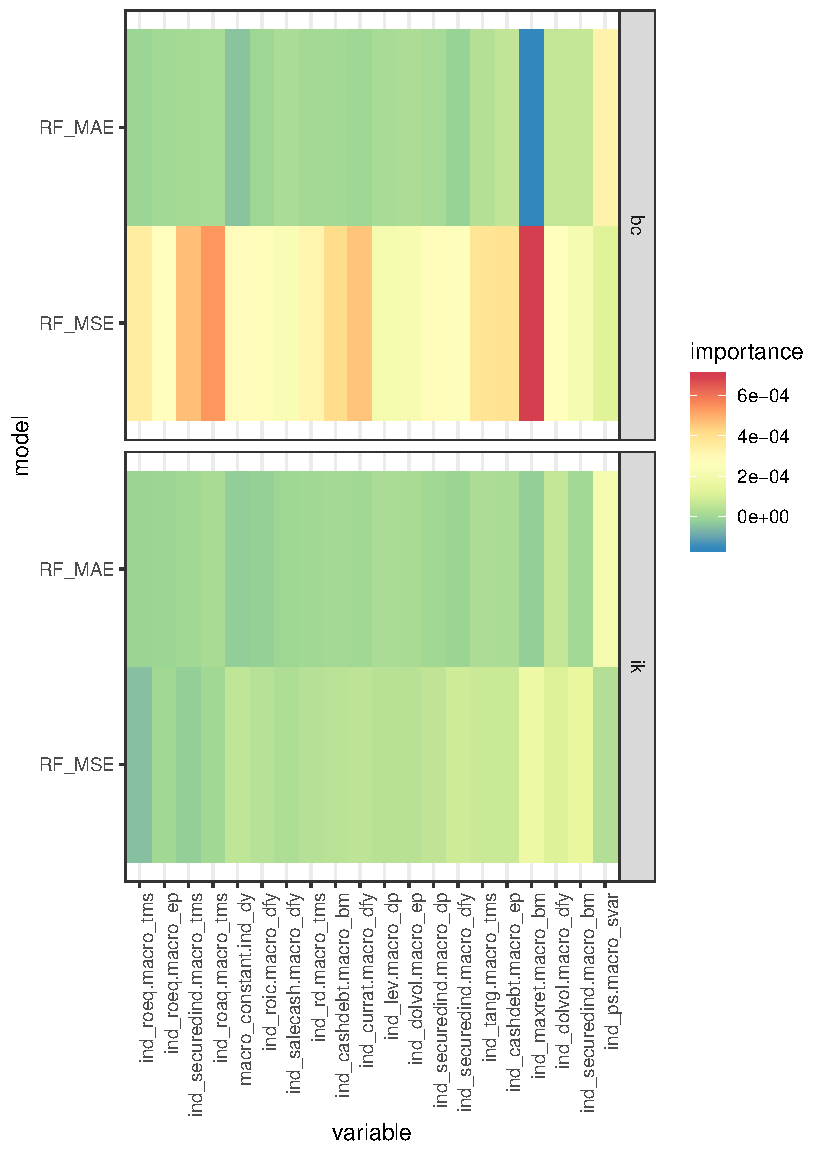
\includegraphics[max size = {\textwidth}{0.35\textheight}]{../../Results/empirical/empirical_vimp.pdf}
	\caption{Empirical study random forest vimps}
\end{figure}
\FloatBarrier
%%%%%%%%%%%%%%%%%%%%%%%%%%%%%%%%%%%%%%%%%%%%%%
%% Missing Data Threshold Robustness Check
% Loss Stats

\paragraph{Missing threshold} We consider changing the missing data threshold to be 10\% - that is, any regressors with over 10\% missing data were omitted before being imputed.
\FloatBarrier
\begin{table}[H]
\centering\begingroup\fontsize{6}{8}\selectfont

\begin{tabular}{cccccccccc}
\toprule
\multicolumn{1}{c}{ } & \multicolumn{3}{c}{Sample 1} & \multicolumn{3}{c}{Sample 2} & \multicolumn{3}{c}{Sample 3} \\
\cmidrule(l{3pt}r{3pt}){2-4} \cmidrule(l{3pt}r{3pt}){5-7} \cmidrule(l{3pt}r{3pt}){8-10}
model & Test MAE & Test MSE & Test $R^2$ & Test MAE & Test MSE & Test $R^2$ & Test MAE & Test MSE & Test $R^2$\\
\midrule
LM.MSE & 0.247457 & 0.130166 & -2.151058 & 0.541089 & 0.700574 & -15.424468 & 0.615714 & 1.188991 & -25.279238\\
LM.MAE & 0.214055 & 0.102848 & -1.489727 & 0.372683 & 0.259976 & -5.094954 & 0.507397 & 0.766373 & -15.93847\\
ELN.MSE & 0.133887 & 0.039947 & 0.032956 & 0.140402 & 0.04277 & -0.002712 & \textbf{0.14433} & \textbf{0.043761} & \textbf{0.032789}\\
ELN.MAE & 0.131338 & 0.040465 & 0.020421 & \textbf{0.137083} & \textbf{0.041804} & \textbf{0.019938} & 0.146589 & 0.045362 & -0.002596\\
RF.MSE & 0.129226 & 0.035869 & 0.131692 & 0.198914 & 0.072749 & -0.705542 & 0.168068 & 0.05777 & -0.276838\\
\addlinespace
RF.MAE & \textbf{0.124319} & \textbf{0.035103} & \textbf{0.150229} & 0.167845 & 0.053578 & -0.256106 & 0.15463 & 0.051594 & -0.140342\\
NN1.MSE & 0.153785 & 0.048726 & -0.179553 & 0.221019 & 0.084867 & -0.98964 & 0.172557 & 0.058354 & -0.289742\\
NN1.MAE & 0.154534 & 0.048854 & -0.18266 & 0.199647 & 0.073699 & -0.727823 & 0.176348 & 0.061359 & -0.356155\\
NN2.MSE & 0.158513 & 0.057061 & -0.381324 & 0.233631 & 0.095004 & -1.227299 & 0.154083 & 0.048353 & -0.068708\\
NN2.MAE & 0.138489 & 0.043364 & -0.049759 & 0.215253 & 0.078792 & -0.847234 & 0.164459 & 0.055049 & -0.216706\\
\addlinespace
NN3.MSE & 0.167392 & 0.058508 & -0.416345 & 0.19754 & 0.071293 & -0.671422 & 0.156873 & 0.049602 & -0.096299\\
NN3.MAE & 0.144457 & 0.045293 & -0.096445 & 0.210372 & 0.077747 & -0.822723 & 0.159841 & 0.05152 & -0.138704\\
NN4.MSE & 0.147989 & 0.047211 & -0.142888 & 0.184277 & 0.064247 & -0.506225 & 0.152214 & 0.048185 & -0.064987\\
NN4.MAE & 0.15851 & 0.052021 & -0.259326 & 0.18643 & 0.063032 & -0.477746 & 0.177651 & 0.064046 & -0.415562\\
NN5.MSE & 0.153187 & 0.050053 & -0.211683 & 0.181622 & 0.060313 & -0.413989 & 0.161028 & 0.051221 & -0.132095\\
\addlinespace
NN5.MAE & 0.149496 & 0.050779 & -0.229251 & 0.165726 & 0.053988 & -0.265712 & 0.156151 & 0.049772 & -0.100061\\
\bottomrule
\end{tabular}
\endgroup{}
\end{table}
\FloatBarrier
%% Factor Importance
\begin{figure}
	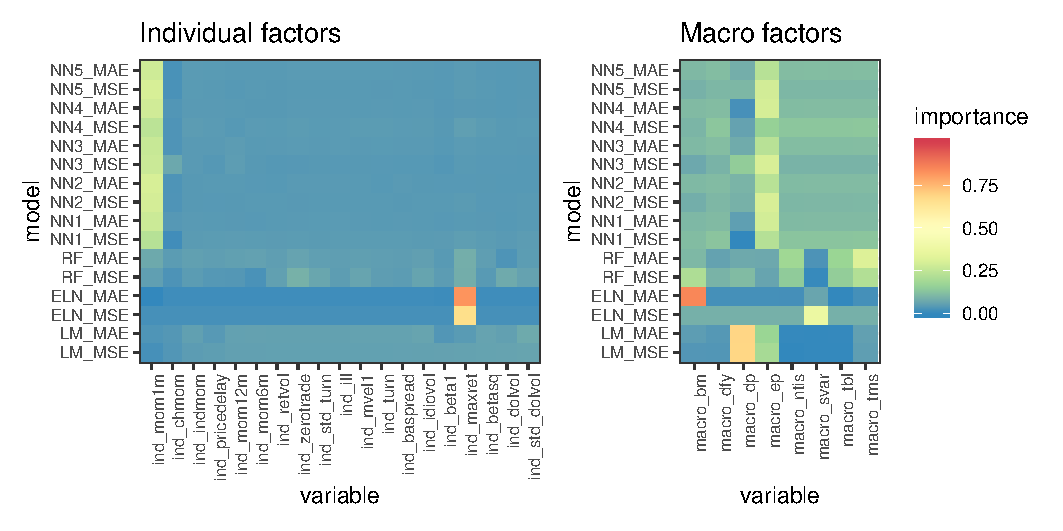
\includegraphics[max size = {\textwidth}{0.35\textheight}]{../../Results/empirical_missing_threshold/empirical_all_sample_vi.pdf}
	\caption{Missing Data Threshold Robustness Check Factor Importance}
\end{figure}

%% RF Vimps
\begin{figure}
	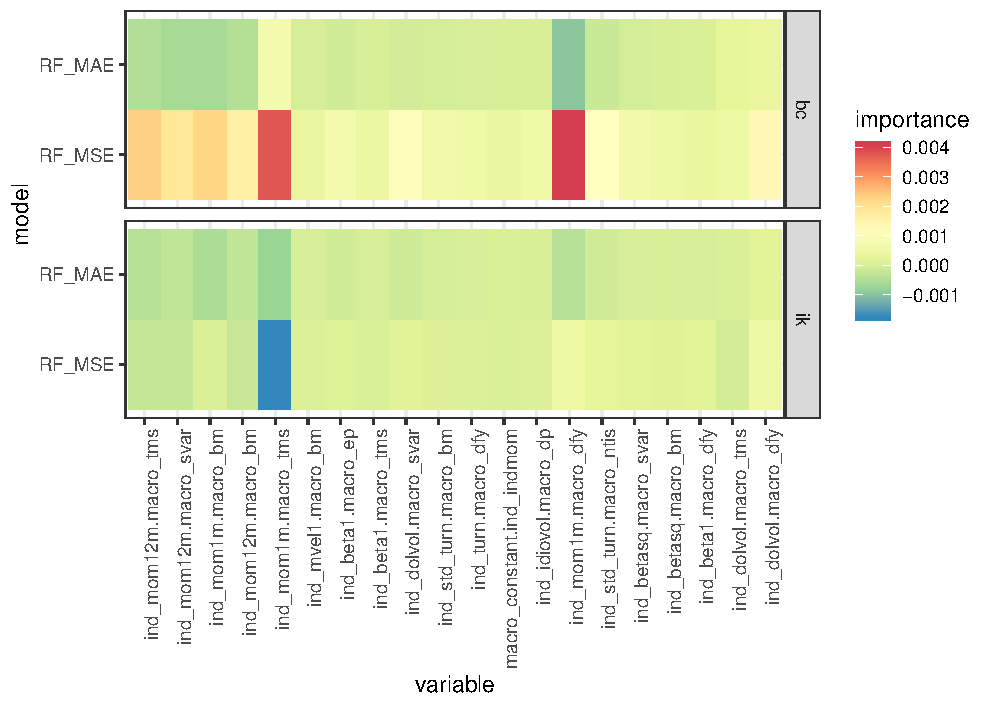
\includegraphics[max size = {\textwidth}{0.35\textheight}]{../../Results/empirical_missing_threshold/empirical_vimp.pdf}
	\caption{Missing Data Threshold Robustness Check RF VIMP}
\end{figure}
\FloatBarrier
\paragraph{Train/validation schemes}%% 
We consider training:validation length ratios of 1:1 and 1:2 in addition to 1.5:1 in the main study.
%%%%%%%%%%%%%%%%%%%%%%%%%%%%%%%%%%%%%%%%%%
%% Train:Validation 1:1
%%%%%%%%%%%%%%%%%%%%%%%%%%%%%%%%%%%%%%%%%%

%% Loss Stats
\FloatBarrier
\begin{table}

\caption{\label{tab:}Train:Validation 1:1 Robustness Check Loss Statistics}
\centering
\fontsize{6}{8}\selectfont
\begin{tabular}[t]{cccccccccc}
\toprule
\multicolumn{1}{c}{ } & \multicolumn{3}{c}{Sample 1} & \multicolumn{3}{c}{Sample 2} & \multicolumn{3}{c}{Sample 3} \\
\cmidrule(l{3pt}r{3pt}){2-4} \cmidrule(l{3pt}r{3pt}){5-7} \cmidrule(l{3pt}r{3pt}){8-10}
model & Test MAE & Test MSE & Test $R^2$ & Test MAE & Test MSE & Test $R^2$ & Test MAE & Test MSE & Test $R^2$\\
\midrule
LM.MSE & 0.915703 & 2.495094 & -59.401029 & 0.717 & 1.553454 & -35.419641 & 0.451206 & 0.375505 & -7.299459\\
LM.MAE & 0.751551 & 1.583265 & -37.32754 & 0.469831 & 0.524686 & -11.300895 & 0.675112 & 1.105759 & -23.43964\\
ELN.MSE & 0.134609 & \textbf{0.040072} & \textbf{0.029933} & 0.141434 & 0.043169 & -0.012055 & \textbf{0.144375} & \textbf{0.043705} & \textbf{0.034019}\\
ELN.MAE & \textbf{0.131668} & 0.040748 & 0.013583 & \textbf{0.137494} & \textbf{0.042135} & \textbf{0.012178} & 0.146776 & 0.045753 & -0.01123\\
RF.MSE & 0.155282 & 0.046655 & -0.129427 & 0.210936 & 0.078006 & -0.828784 & 0.229147 & 0.092622 & -1.047155\\
RF.MAE & 0.13882 & 0.04016 & 0.027805 & 0.185338 & 0.063217 & -0.482087 & 0.182753 & 0.063873 & -0.411736\\
NN1.MSE & 0.218129 & 0.087699 & -1.123002 & 0.238606 & 0.110201 & -1.583582 & 0.260721 & 0.120908 & -1.672321\\
NN1.MAE & 0.202259 & 0.072844 & -0.763409 & 0.205092 & 0.073567 & -0.724721 & 0.239051 & 0.096477 & -1.132346\\
NN2.MSE & 0.239446 & 0.101312 & -1.452556 & 0.206109 & 0.078412 & -0.838305 & 0.228591 & 0.095126 & -1.102488\\
NN2.MAE & 0.19141 & 0.068261 & -0.652455 & 0.184095 & 0.062366 & -0.462125 & 0.220087 & 0.086888 & -0.920403\\
NN3.MSE & 0.193117 & 0.069206 & -0.675336 & 0.193859 & 0.070747 & -0.658609 & 0.205093 & 0.076497 & -0.690745\\
NN3.MAE & 0.191596 & 0.066926 & -0.620138 & 0.176555 & 0.060022 & -0.407183 & 0.234768 & 0.091003 & -1.011359\\
NN4.MSE & 0.191361 & 0.07068 & -0.71101 & 0.175311 & 0.059253 & -0.389136 & 0.18148 & 0.061718 & -0.364096\\
NN4.MAE & 0.139659 & 0.041096 & 0.005158 & 0.179318 & 0.05976 & -0.401027 & 0.188921 & 0.066144 & -0.461932\\
NN5.MSE & 0.17209 & 0.056982 & -0.379418 & 0.164756 & 0.054398 & -0.275325 & 0.202012 & 0.074051 & -0.636691\\
NN5.MAE & 0.170945 & 0.056029 & -0.356356 & 0.180669 & 0.059697 & -0.399552 & 0.189149 & 0.065921 & -0.456988\\
\bottomrule
\end{tabular}
\end{table}
\FloatBarrier

%% Factor Importance
\begin{figure}
	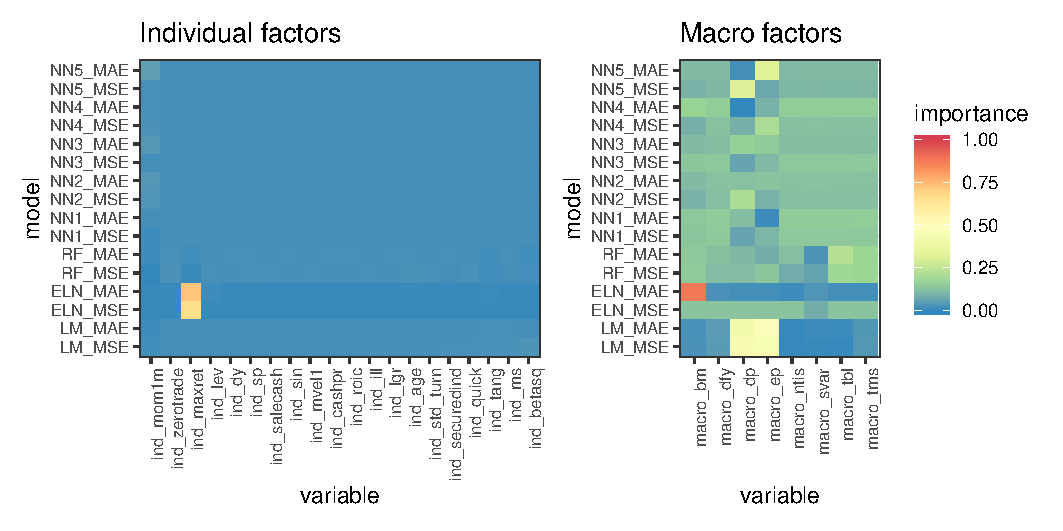
\includegraphics[max size = {\textwidth}{0.35\textheight}]{../../Results/empirical_train_valid_1/empirical_all_sample_vi.pdf}
	\caption{{Train:Validation = 1:1 Robustness Check Factor Importance}}
\end{figure}

%% RF Vimps
\begin{figure}
	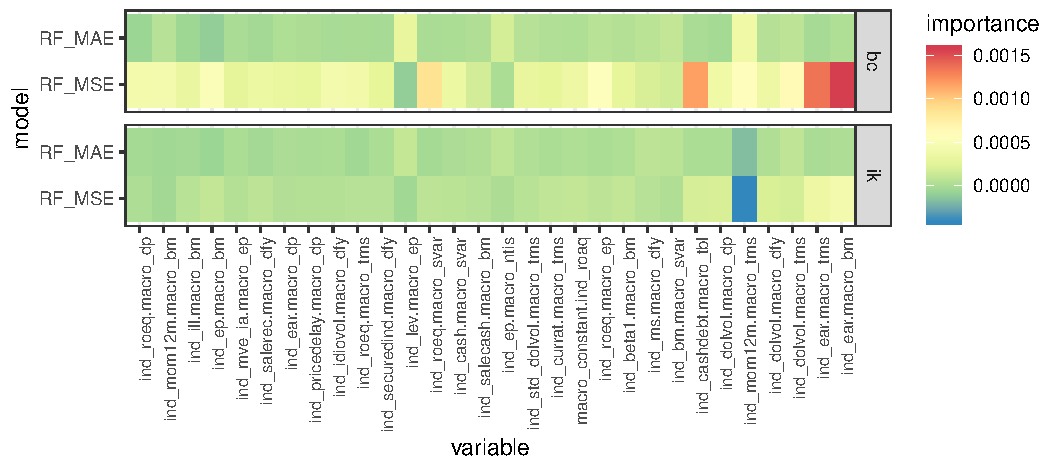
\includegraphics[max size = {\textwidth}{0.35\textheight}]{../../Results/empirical_train_valid_1/empirical_vimp.pdf}
	\caption{{Train:Validation = 1:1 Robustness Check RF VIMP}}
\end{figure}
\FloatBarrier
%%%%%%%%%%%%%%%%%%%%%%%%%%%%%%%%%%%%%%%%%%
%% Train:Validation 2:1
%%%%%%%%%%%%%%%%%%%%%%%%%%%%%%%%%%%%%%%%%%
%% Loss Stats
\FloatBarrier
\begin{table}

\caption{\label{tab:}Train:Validation 2:1 Robustness Check Loss Statistics}
\centering
\fontsize{6}{8}\selectfont
\begin{tabular}[t]{cccccccccc}
\toprule
\multicolumn{1}{c}{ } & \multicolumn{3}{c}{Sample 1} & \multicolumn{3}{c}{Sample 2} & \multicolumn{3}{c}{Sample 3} \\
\cmidrule(l{3pt}r{3pt}){2-4} \cmidrule(l{3pt}r{3pt}){5-7} \cmidrule(l{3pt}r{3pt}){8-10}
model & Test MAE & Test MSE & Test $R^2$ & Test MAE & Test MSE & Test $R^2$ & Test MAE & Test MSE & Test $R^2$\\
\midrule
LM.MSE & 0.277087 & 0.164599 & -2.98459 & 0.383421 & 0.31299 & -6.337839 & 0.523418 & 0.740288 & -15.361936\\
LM.MAE & 0.246936 & 0.147979 & -2.582262 & 0.277044 & 0.161215 & -2.779579 & 0.487285 & 0.631575 & -12.95915\\
ELN.MSE & 0.133715 & 0.039919 & 0.033647 & 0.139723 & 0.042525 & 0.003028 & \textbf{0.145034} & \textbf{0.044306} & \textbf{0.020752}\\
ELN.MAE & 0.131237 & 0.040361 & 0.022952 & \textbf{0.137205} & \textbf{0.041858} & \textbf{0.018674} & 0.174408 & 0.064513 & -0.425873\\
RF.MSE & 0.130808 & 0.036982 & 0.104754 & 0.162762 & 0.051118 & -0.198417 & 0.155264 & 0.048661 & -0.075516\\
RF.MAE & \textbf{0.127013} & \textbf{0.036722} & \textbf{0.111033} & 0.146758 & 0.043961 & -0.030633 & 0.168905 & 0.055983 & -0.237348\\
NN1.MSE & 0.155088 & 0.050284 & -0.217281 & 0.165871 & 0.053459 & -0.253309 & 0.181984 & 0.064621 & -0.428262\\
NN1.MAE & 0.159797 & 0.050566 & -0.224107 & 0.163397 & 0.052329 & -0.226828 & 0.181636 & 0.062407 & -0.379326\\
NN2.MSE & 0.155815 & 0.050954 & -0.233492 & 0.168576 & 0.055738 & -0.306745 & 0.170991 & 0.057453 & -0.269824\\
NN2.MAE & 0.148149 & 0.047617 & -0.152709 & 0.166334 & 0.054058 & -0.26734 & 0.163141 & 0.052639 & -0.163436\\
NN3.MSE & 0.154141 & 0.04976 & -0.204586 & 0.166218 & 0.053402 & -0.251967 & 0.169539 & 0.05661 & -0.251204\\
NN3.MAE & 0.142464 & 0.043771 & -0.059594 & 0.154233 & 0.048682 & -0.141321 & 0.184217 & 0.064175 & -0.418401\\
NN4.MSE & 0.166547 & 0.056184 & -0.360092 & 0.150748 & 0.047566 & -0.115162 & 0.168447 & 0.056575 & -0.250437\\
NN4.MAE & 0.150167 & 0.046919 & -0.135802 & 0.16197 & 0.05226 & -0.225199 & 0.171676 & 0.057352 & -0.267598\\
NN5.MSE & 0.155784 & 0.052258 & -0.265047 & 0.139699 & 0.043082 & -0.010018 & 0.166166 & 0.055027 & -0.216219\\
NN5.MAE & 0.161161 & 0.053216 & -0.28825 & 0.149207 & 0.046344 & -0.086511 & 0.149424 & 0.047544 & -0.050824\\
\bottomrule
\end{tabular}
\end{table}
\FloatBarrier
%% Factor Importance
\begin{figure}
	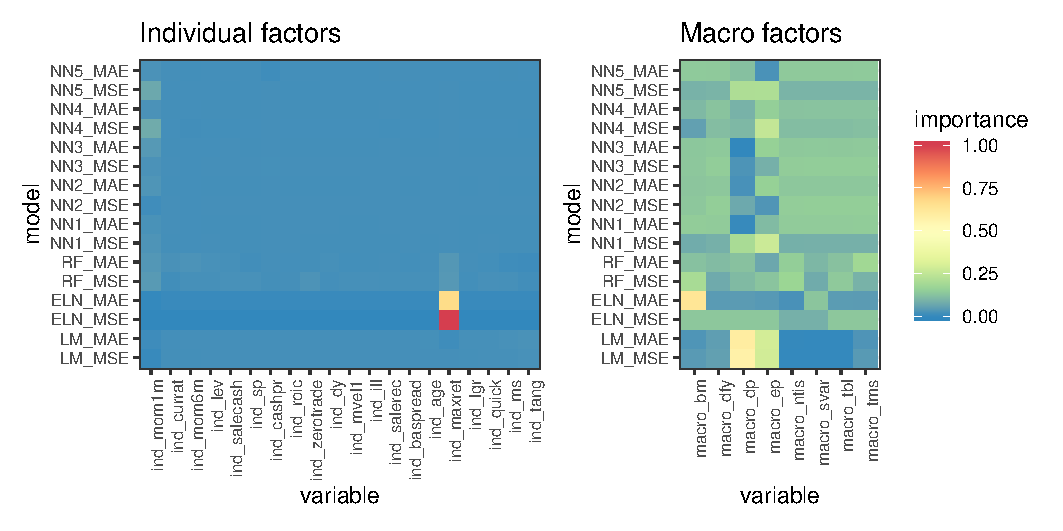
\includegraphics[max size = {\textwidth}{0.35\textheight}]{../../Results/empirical_train_valid_2/empirical_all_sample_vi.pdf}
	\caption{Train:Validation = 2:1 Robustness Check Factor Importance}
\end{figure}
%% RF Vimps
\begin{figure}
	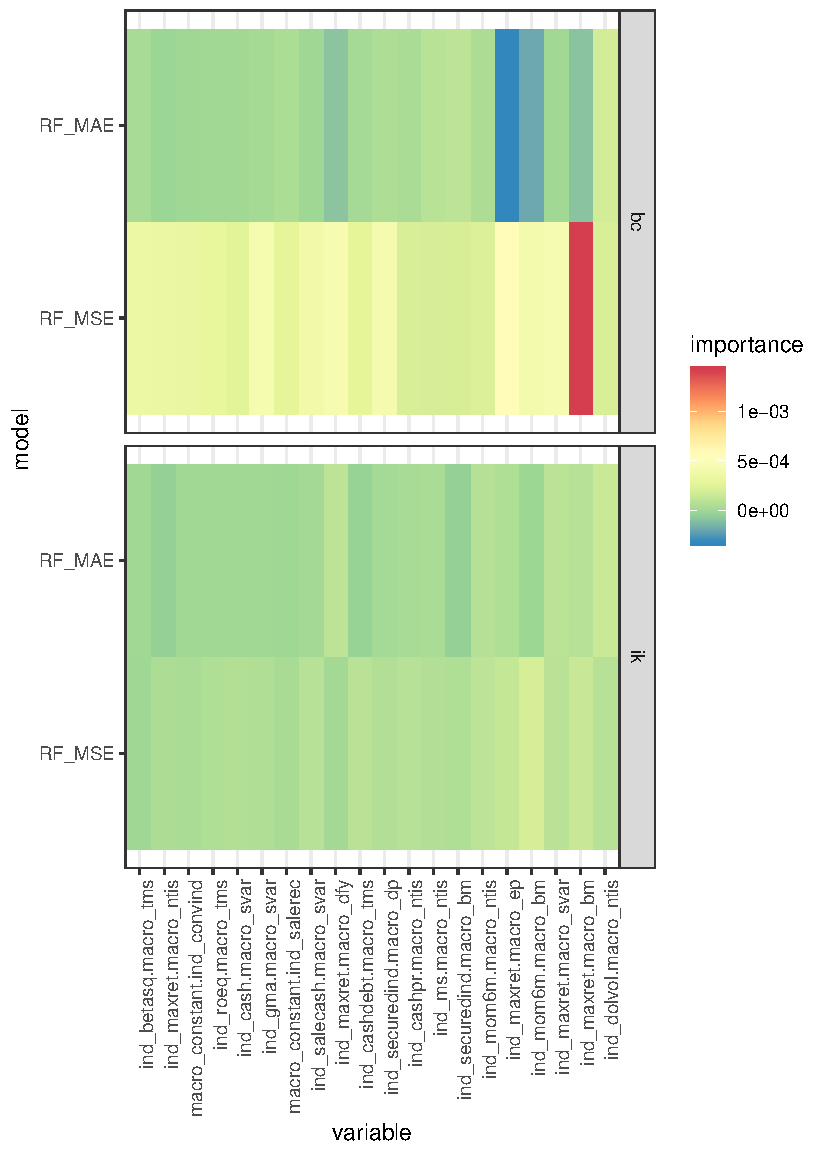
\includegraphics[max size = {\textwidth}{0.35\textheight}]{../../Results/empirical_train_valid_2/empirical_vimp.pdf}
	\caption{Train:Validation = 2:1 Robustness Check RF VIMP}
\end{figure}
\FloatBarrier
%%%%%%%%%%%%%%%%%%%%%%%%%%%%%%%%%%%%%%%%%%
%% Fama French Factors
%%%%%%%%%%%%%%%%%%%%%%%%%%%%%%%%%%%%%%%%%%
\paragraph{Fama French factors} 
We finally consider supplementing our macroeconomic regressor set with the five Fama-French factors. 
%% Loss Stats
\FloatBarrier
\begingroup\fontsize{6}{8}\selectfont

\begin{longtable}{cccccccccc}
\toprule
\multicolumn{1}{c}{ } & \multicolumn{3}{c}{Sample 1} & \multicolumn{3}{c}{Sample 2} & \multicolumn{3}{c}{Sample 3} \\
\cmidrule(l{3pt}r{3pt}){2-4} \cmidrule(l{3pt}r{3pt}){5-7} \cmidrule(l{3pt}r{3pt}){8-10}
model & Test MAE & Test MSE & Test $R^2$ & Test MAE & Test MSE & Test $R^2$ & Test MAE & Test MSE & Test $R^2$\\
\midrule
\endfirsthead
\multicolumn{10}{@{}l}{}\\
\toprule
\multicolumn{1}{c}{ } & \multicolumn{3}{c}{Sample 1} & \multicolumn{3}{c}{Sample 2} & \multicolumn{3}{c}{Sample 3} \\
\cmidrule(l{3pt}r{3pt}){2-4} \cmidrule(l{3pt}r{3pt}){5-7} \cmidrule(l{3pt}r{3pt}){8-10}
model & Test MAE & Test MSE & Test $R^2$ & Test MAE & Test MSE & Test $R^2$ & Test MAE & Test MSE & Test $R^2$\\
\midrule
\endhead
\
\endfoot
\bottomrule
\endlastfoot
LM.MSE & 0.288636 & 0.182966 & -3.42923 & 0.367636 & 0.264918 & -5.210825 & 1.101604 & 5.012469 & -109.78624\\
LM.MAE & 0.280535 & 0.179777 & -3.352038 & 0.376163 & 0.279476 & -5.552114 & 1.25341 & 7.06036 & -155.048996\\
ELN.MSE & 0.13383 & 0.039956 & 0.032746 & 0.14022 & 0.0427 & -0.00107 & \textbf{0.144472} & \textbf{0.043852} & \textbf{0.030769}\\
ELN.MAE & \textbf{0.128936} & \textbf{0.039665} & \textbf{0.039798} & \textbf{0.13716} & \textbf{0.042144} & \textbf{0.011965} & 0.172148 & 0.063154 & -0.395841\\
RF.MSE & 0.146318 & 0.042607 & -0.031434 & 0.151137 & 0.047091 & -0.104011 & 0.177125 & 0.064664 & -0.429221\\
\addlinespace
RF.MAE & 0.138266 & 0.04005 & 0.030475 & 0.138714 & 0.042246 & 0.009583 & 0.152068 & 0.048488 & -0.071698\\
NN1.MSE & 0.168063 & 0.055354 & -0.340017 & 0.192143 & 0.068904 & -0.61541 & 0.275195 & 0.138165 & -2.053731\\
NN1.MAE & 0.161596 & 0.051507 & -0.246873 & 0.199416 & 0.068181 & -0.598444 & 0.23054 & 0.093434 & -1.065082\\
NN2.MSE & 0.169842 & 0.056899 & -0.377415 & 0.179733 & 0.058966 & -0.382416 & 0.252929 & 0.117102 & -1.588199\\
NN2.MAE & 0.155816 & 0.046809 & -0.133147 & 0.185008 & 0.060854 & -0.426679 & 0.219342 & 0.085115 & -0.881213\\
\addlinespace
NN3.MSE & 0.1621 & 0.053165 & -0.287008 & 0.182996 & 0.059643 & -0.398278 & 0.232226 & 0.099353 & -1.195903\\
NN3.MAE & 0.161255 & 0.050737 & -0.228237 & 0.191625 & 0.064676 & -0.516291 & 0.218355 & 0.085297 & -0.885238\\
NN4.MSE & 0.166036 & 0.055575 & -0.345349 & 0.191589 & 0.066207 & -0.552182 & 0.23417 & 0.097348 & -1.151607\\
NN4.MAE & 0.148375 & 0.045227 & -0.094843 & 0.168623 & 0.054176 & -0.270114 & 0.20837 & 0.077667 & -0.7166\\
NN5.MSE & 0.147379 & 0.044503 & -0.077315 & 0.166006 & 0.054935 & -0.287914 & 0.20667 & 0.077866 & -0.721013\\
\addlinespace
NN5.MAE & 0.150541 & 0.045723 & -0.106868 & 0.172466 & 0.055402 & -0.298865 & 0.218796 & 0.084938 & -0.877301\\*
\end{longtable}
\endgroup{}
\FloatBarrier

%% Factor Importance
\begin{figure}
	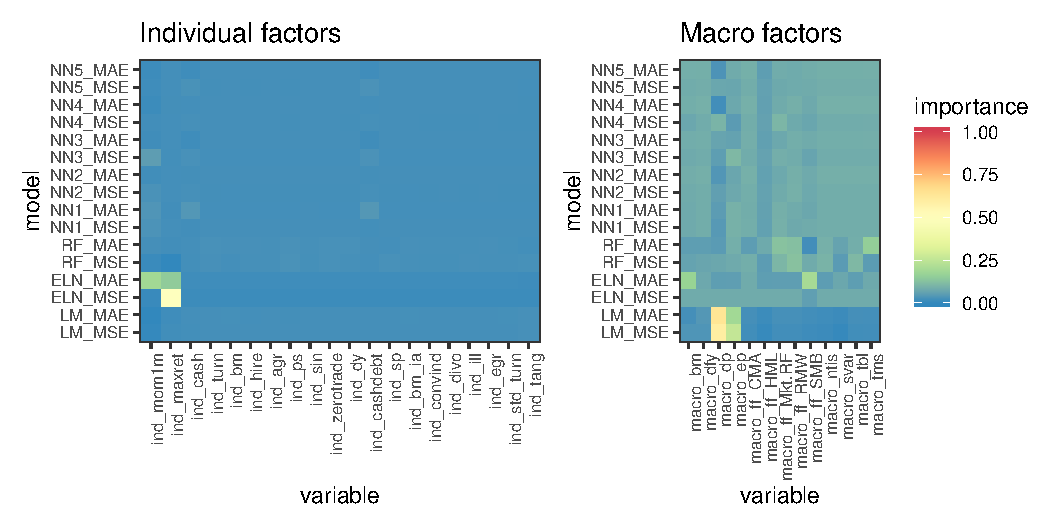
\includegraphics[max size = {\textwidth}{0.35\textheight}]{../../Results/empirical_ff/empirical_all_sample_vi.pdf}
	\caption{Fama French Factors Robustness Check Factor Importance}
\end{figure}

%% RF Vimps
\begin{figure}
	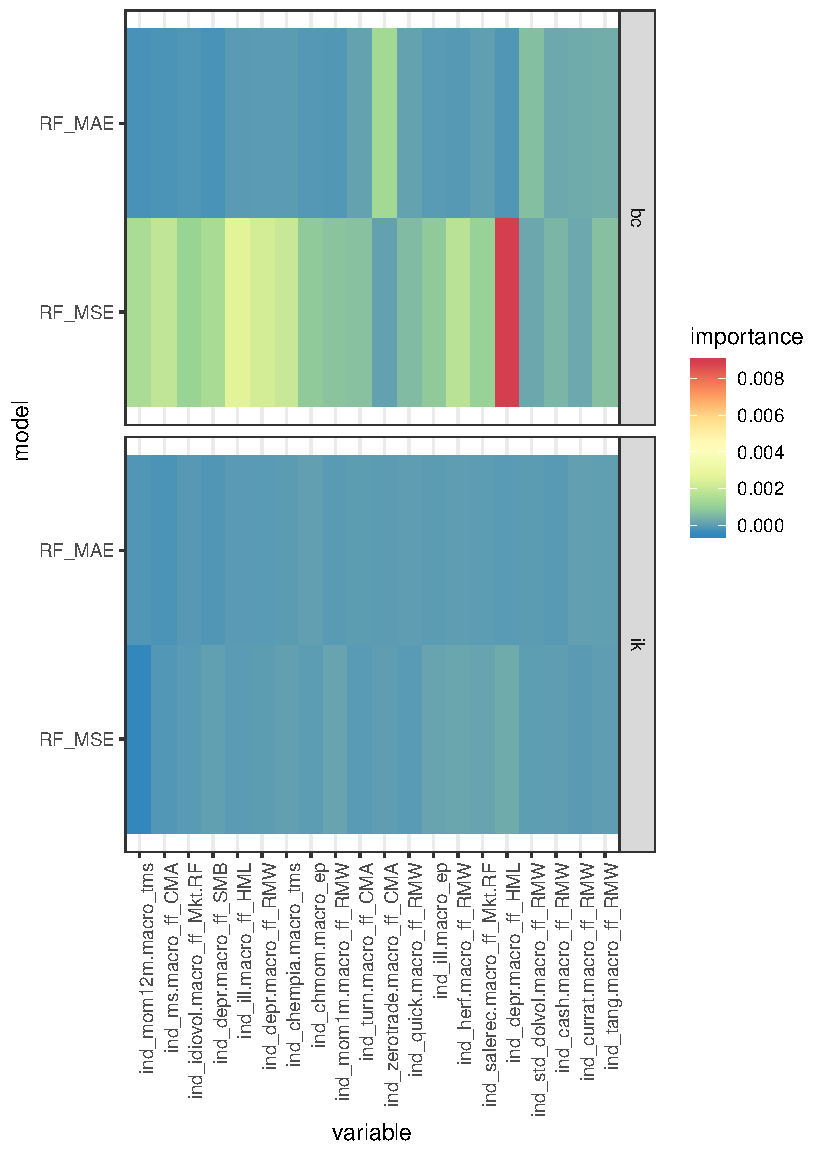
\includegraphics[max size = {\textwidth}{0.35\textheight}]{../../Results/empirical_ff/empirical_vimp.pdf}
	\caption{Fama French Factors Robustness Check RF VIMP}
\end{figure}
\FloatBarrier
\end{document}